\chapter{MPC with Learning\texorpdfstring{$^{(*)}$}{(*)}}
\label{chap:learning_mpc}

\begin{quote}
	\textit{``All models are wrong, but some are useful.''} \\
	\hfill --- \emph{George E.\,P.\ Box} (1976)
\end{quote}

Every MPC controller we have built so far starts from the same assumption: a known, accurate model $x_{k+1} = Ax_k + Bu_k$. Chapters~\ref{chap:lqr}--\ref{chap:output_fb_mpc} derive the optimal control law, the estimator, and the constraint-handling machinery on top of this model. Tube MPC relaxes the assumption slightly, admitting bounded disturbances, but still requires the system matrices $A$ and $B$ and a known disturbance bound $\mathcal{W}$.

In many practical situations, however, the model is the bottleneck. Three distinct problems arise:
\begin{enumerate}
	\item \emph{Model inaccuracy.} The identified $A$ and $B$ are approximate. The true dynamics contain terms the model ignores---friction, aerodynamic drag, thermal coupling.
	\item \emph{Model incompleteness.} Part of the dynamics is entirely unknown. A robot grasping an unfamiliar object does not know the object's mass or friction coefficient.
	\item \emph{No model at all.} For some systems---biological processes, soft robots, complex chemical reactors---first-principles modelling is prohibitively difficult. Only input--output data is available.
\end{enumerate}

This chapter introduces methods that combine \emph{learning from data} with \emph{MPC}. The central question is: \emph{how can we use measured data to replace, correct, or bypass the model, while retaining the constraint-handling and optimality guarantees that make MPC attractive?}

\section{Three Paradigms for Learning in MPC}
\label{sec:learning_paradigms}

The methods in this chapter fall into three families, distinguished by \emph{what} is learned.

\begin{defnbox}{Three Paradigms}
	\begin{enumerate}
		\item \emph{Model Learning.} Learn the unknown dynamics $f(x,u)$---or a correction to a nominal model---from data. Then use the learned model inside a standard MPC formulation.\\
		\emph{Methods:} Gaussian Process MPC (Section~\ref{sec:gpmpc}), Neural Network MPC (Section~\ref{sec:nnmpc}).

		\item \emph{Data-Driven Control.} Use trajectory data to construct a linear prediction model or bypass system identification entirely.\\
		\emph{Methods:} Koopman/EDMD MPC (Section~\ref{sec:koopman}), DeePC (Section~\ref{sec:deepc}).\\
		\emph{Note:} Koopman/EDMD identifies matrices $(A_K, B_K)$ from data---an indirect data-driven approach. DeePC uses data directly without ever forming an explicit model.

		\item \emph{Policy Learning.} Use closed-loop experience from previous task executions to improve the MPC policy itself---expanding the safe region and reducing cost over repeated attempts.\\
		\emph{Methods:} Learning MPC (Section~\ref{sec:lmpc}).
	\end{enumerate}
\end{defnbox}

\begin{notebox}{Connection to Earlier Chapters}
	Each approach builds on tools already developed in these notes:
	\begin{center}
		\begin{tabular}{l l}
			\toprule
			\emph{Approach} & \emph{Prerequisites} \\
			\midrule
			GP-MPC & Ch.\,6 (Bayesian estimation), Ch.\,7 (constrained MPC), Tube MPC (uncertainty) \\
			Koopman MPC & Ch.\,3 (state-space), Ch.\,5 (QP/LQR), Ch.\,7 (linear MPC) \\
			DeePC & Ch.\,2 (optimisation/YALMIP), Ch.\,7 (MPC formulation) \\
			LMPC & Ch.\,7 (terminal sets, recursive feasibility) \\
			\bottomrule
		\end{tabular}
	\end{center}
\end{notebox}

\begin{alertbox}{When is learning necessary?}
	Not every MPC application needs learning. If a first-principles model is available and accurate, standard MPC (Chapter~7) or Tube MPC are preferable---they are simpler to implement and their guarantees are better understood. Learning is most valuable when:
	\begin{itemize}[noitemsep]
		\item The model is too expensive or too difficult to derive from physics.
		\item The system changes over time (wear, ageing, varying loads).
		\item The disturbance structure is unknown or state-dependent, so that fixed bounds $\mathcal{W}$ are overly conservative.
	\end{itemize}
\end{alertbox}

Figure~\ref{fig:learning_taxonomy} summarises the three paradigms and the methods covered in this chapter.

\begin{figure}[ht]
	\centering
	\resizebox{\linewidth}{!}{%
	\begin{tikzpicture}[
		>=Stealth,
		paradigm/.style={draw, rounded corners=4pt, fill=blue!12,
			text width=3.0cm, minimum height=1.0cm, align=center,
			font=\small\bfseries},
		method/.style={draw, rounded corners=3pt, fill=orange!12,
			text width=2.2cm, minimum height=0.8cm, align=center,
			font=\small},
		root/.style={draw, rounded corners=6pt, fill=gray!15,
			text width=4.8cm, minimum height=1.0cm, align=center,
			font=\normalsize\bfseries},
	]
		% Root
		\node[root] at (0,0) (root) {Learning-Based MPC};

		% Paradigms — centres above their child groups
		\node[paradigm] at (-5.25,-1.7) (p1) {Model Learning};
		\node[paradigm] at (1.75,-1.7)  (p2) {Data-Driven\\Control};
		\node[paradigm] at (7.0,-1.7)   (p3) {Policy Learning};

		% Arrows from root to paradigms
		\draw[->, thick] (root.south) -- ++(0,-0.35) -| (p1.north);
		\draw[->, thick] (root.south) -- ++(0,-0.35) -| (p2.north);
		\draw[->, thick] (root.south) -- ++(0,-0.35) -| (p3.north);

		% Methods — 5 leaf nodes with 3.5cm centre-to-centre spacing (≈1cm gap)
		\node[method] at (-7.0,-4.6) (m1a) {GP-MPC\\{\scriptsize (Sec.~\ref{sec:gpmpc})}};
		\node[method] at (-3.5,-4.6) (m1b) {NN-MPC\\{\scriptsize (Sec.~\ref{sec:nnmpc})}};
		\node[method] at (0.0,-4.6)  (m2a) {Koopman MPC\\{\scriptsize (Sec.~\ref{sec:koopman})}};
		\node[method] at (3.5,-4.6)  (m2b) {DeePC\\{\scriptsize (Sec.~\ref{sec:deepc})}};
		\node[method] at (7.0,-4.6)  (m3a) {LMPC\\{\scriptsize (Sec.~\ref{sec:lmpc})}};

		% Arrows from paradigms to methods
		\draw[->, thick] (p1.south) -- ++(0,-0.35) -| (m1a.north);
		\draw[->, thick] (p1.south) -- ++(0,-0.35) -| (m1b.north);
		\draw[->, thick] (p2.south) -- ++(0,-0.35) -| (m2a.north);
		\draw[->, thick] (p2.south) -- ++(0,-0.35) -| (m2b.north);
		\draw[->, thick] (p3.south) -- (m3a.north);

		% Annotations: QP vs NLP
		\node[below=0.25cm of m1a, font=\scriptsize\itshape, text=red!70!black] {NLP};
		\node[below=0.25cm of m1b, font=\scriptsize\itshape, text=red!70!black] {NLP (severe)};
		\node[below=0.25cm of m2a, font=\scriptsize\itshape, text=blue!70!black] {QP};
		\node[below=0.25cm of m2b, font=\scriptsize\itshape, text=blue!70!black] {QP};
		\node[below=0.25cm of m3a, font=\scriptsize\itshape, text=black!60] {QP or NLP};
	\end{tikzpicture}%
	}
	\caption{Taxonomy of learning-based MPC methods. Model learning approaches (GP-MPC, NN-MPC) learn the unknown dynamics and embed the learned model in MPC. Data-driven approaches (Koopman MPC, DeePC) use data directly, preserving the QP structure of linear MPC. Policy learning (LMPC) improves the controller from repeated task executions. The annotation below each method indicates whether the resulting online optimisation is a convex QP or a non-convex NLP.}
	\label{fig:learning_taxonomy}
\end{figure}


%% ============================================================
%%  SECTION 2: GAUSSIAN PROCESS MPC
%% ============================================================
\section{Gaussian Process MPC}
\label{sec:gpmpc}

Suppose we have a nominal model $x_{k+1} = Ax_k + Bu_k$ that captures the dominant dynamics, but the true system contains an additional unknown term:
\begin{equation}\label{eq:residual_model}
	x_{k+1} = Ax_k + Bu_k + g(x_k, u_k)
\end{equation}
where $g \colon \mathbb{R}^n \times \mathbb{R}^m \to \mathbb{R}^n$ is an unknown function representing unmodelled dynamics. The idea behind GP-MPC is to learn $g$ from data as a \emph{Gaussian process}---a probabilistic model that provides not only a best-guess prediction but also a measure of confidence. This confidence is then used to tighten the MPC constraints adaptively: more in regions where data is sparse and the model is uncertain, less where data is dense and the model is reliable.

\subsection{Gaussian Process Regression}
\label{sec:gp_regression}

A Gaussian process is a tool for learning an unknown function from noisy observations. The reader needs basic probability from Appendix~B; in particular, the conditional multivariate Gaussian (Section~\ref{sec:app_cond_gauss}) is the mathematical foundation of GP prediction, and the chance-constraint conversion (Section~\ref{sec:app_chance_constraints}) is used for constraint tightening in Section~\ref{sec:gpmpc_formulation}.

\subsubsection*{The Setup}

We have $T$ noisy observations of an unknown scalar function $f$:
\[
y_i = f(x_i) + \varepsilon_i, \qquad \varepsilon_i \sim \mathcal{N}(0, \sigma_n^2), \qquad i = 1, \ldots, T
\]
where $x_i$ is the input (which may be a vector), $y_i$ is the observed output, and $\varepsilon_i$ is independent Gaussian noise with variance $\sigma_n^2$. Given these $T$ pairs, we want to predict $f(x_*)$ at a new test point $x_*$.

\subsubsection*{The Gaussian Process Prior}

A parametric model (e.g.\ a polynomial) commits to a fixed functional form and learns its coefficients. A Gaussian process takes a different approach: it places a probability distribution directly over \emph{functions}.

\begin{defnbox}{Definition: Gaussian Process}
	A \emph{Gaussian process} (GP) is a collection of random variables, any finite subset of which has a joint Gaussian distribution. A GP is fully specified by its \emph{mean function} $m(x)$ and \emph{covariance function} (or \emph{kernel}) $k(x, x')$:
	\[
	f \sim \mathcal{GP}\bigl(m(x),\; k(x, x')\bigr)
	\]
	For any finite set of inputs $\{x_1, \ldots, x_T\}$, the function values $[f(x_1), \ldots, f(x_T)]^\top$ are jointly Gaussian with mean $[m(x_1), \ldots, m(x_T)]^\top$ and covariance matrix $K_{ij} = k(x_i, x_j)$.
\end{defnbox}

We typically set $m(x) = 0$ (the prior mean is zero, meaning no prior bias), so that all structure in the function is captured by the kernel $k(x, x')$.

\subsubsection*{The Kernel}

The kernel encodes our assumptions about the unknown function: how smooth it is, how fast it varies, and over what length scales. The most common choice is the \emph{squared exponential} (SE) kernel:
\begin{equation}\label{eq:se_kernel}
	k(x, x') = \sigma_f^2 \exp\!\left(-\frac{\|x - x'\|^2}{2\ell^2}\right)
\end{equation}
This kernel has two hyperparameters:
\begin{itemize}[noitemsep]
	\item $\sigma_f^2$ (\emph{signal variance}): controls the overall amplitude of the function. Larger $\sigma_f$ allows the function to take larger values.
	\item $\ell$ (\emph{length scale}): controls how quickly the function can change. A small $\ell$ permits rapid variation; a large $\ell$ enforces smooth, slowly varying behaviour.
\end{itemize}
When two inputs $x$ and $x'$ are close ($\|x - x'\| \ll \ell$), the kernel is close to $\sigma_f^2$, meaning the function values are highly correlated. When they are far apart ($\|x - x'\| \gg \ell$), the kernel approaches zero and the function values are nearly independent.

\subsubsection*{The Prediction Equations}

Given training inputs $\{x_1, \ldots, x_T\}$, observations $y = [y_1, \ldots, y_T]^\top$, and a test point $x_*$, the GP posterior is Gaussian with:
\begin{align}
	\mu_*(x_*) &= k_*^\top \bigl(K + \sigma_n^2 I\bigr)^{-1} y \label{eq:gp_mean} \\[4pt]
	\sigma_*^2(x_*) &= k(x_*, x_*) - k_*^\top \bigl(K + \sigma_n^2 I\bigr)^{-1} k_* \label{eq:gp_var}
\end{align}
where:
\begin{itemize}[noitemsep]
	\item $K \in \mathbb{R}^{T \times T}$ is the \emph{Gram matrix} with entries $K_{ij} = k(x_i, x_j)$.
	\item $k_* = [k(x_*, x_1), \ldots, k(x_*, x_T)]^\top \in \mathbb{R}^T$ is the vector of kernel evaluations between the test point and all training points.
	\item $\sigma_n^2$ is the noise variance.
\end{itemize}

\begin{summarybox}{GP Prediction Recipe}
	Given training data $\{(x_i, y_i)\}_{i=1}^T$ and a test input $x_*$:
	\begin{enumerate}[noitemsep]
		\item Build the Gram matrix $K$ and the test kernel vector $k_*$.
		\item Compute $\alpha = (K + \sigma_n^2 I)^{-1}y$ (solve a linear system---do not invert the matrix explicitly).
		\item The \emph{predicted mean} is $\mu_* = k_*^\top \alpha$.
		\item The \emph{predicted variance} is $\sigma_*^2 = k(x_*,x_*) - k_*^\top (K + \sigma_n^2 I)^{-1}k_*$.
	\end{enumerate}
	The mean $\mu_*$ is the best prediction. The interval $\mu_* \pm 2\sigma_*$ is a 95\% confidence band.
\end{summarybox}

\begin{examplebox}{GP Regression on a Scalar Function}
	We observe 10 noisy samples from $f(x) = \sin(x)$ on the interval $[0, 2\pi]$:
	\[
	y_i = \sin(x_i) + \varepsilon_i, \qquad \varepsilon_i \sim \mathcal{N}(0, 0.04), \qquad i = 1, \ldots, 10
	\]
	We use the SE kernel~\eqref{eq:se_kernel} with $\sigma_f = 1$, $\ell = 1$, and $\sigma_n = 0.2$.

	\solution

	For a test point $x_* = 1.5$:
	\begin{enumerate}
		\item Compute the $10 \times 10$ Gram matrix $K$ using $k(x_i, x_j) = \exp\bigl(-\frac{(x_i - x_j)^2}{2}\bigr)$.
		\item Compute $k_* \in \mathbb{R}^{10}$, where each entry is $k(1.5, x_i)$.
		\item Solve the linear system $(K + 0.04\,I)\,\alpha = y$.
		\item The predicted mean is $\mu_* = k_*^\top \alpha$.
		\item The predicted variance is $\sigma_*^2 = 1 - k_*^\top (K + 0.04\,I)^{-1}k_*$.
	\end{enumerate}

	The resulting mean $\mu_*$ will be close to $\sin(1.5) \approx 0.997$, and the variance $\sigma_*^2$ will be small because $x_* = 1.5$ is close to several training points. In regions far from any training data, the variance grows, reflecting genuine uncertainty.

The following MATLAB script implements this example.

\begin{lstlisting}[language=Matlab, caption={GP regression for $f(x)=\sin(x)$ from noisy data.}]
% 1. Training Data
rng(42);
T  = 10;
X  = sort(2*pi*rand(T,1));
sn = 0.2;
y  = sin(X) + sn*randn(T,1);

% 2. Kernel Hyperparameters
sf = 1;  ell = 1;  sn2 = sn^2;

% 3. Kernel Function
kSE = @(xa,xb) sf^2*exp(-0.5*(xa-xb').^2/ell^2);

% 4. Gram Matrix and Alpha
K     = kSE(X, X);
alpha = (K + sn2*eye(T)) \ y;

% 5. Predictions on a Dense Grid
Xstar  = linspace(0, 2*pi, 200)';
Kstar  = kSE(Xstar, X);
Kss    = kSE(Xstar, Xstar);
mu     = Kstar * alpha;
V      = Kss - Kstar * ((K + sn2*eye(T)) \ Kstar');
sig    = sqrt(diag(V));

% 6. Plot
figure; hold on;
fill([Xstar; flipud(Xstar)], ...
     [mu+2*sig; flipud(mu-2*sig)], ...
     [0.8 0.9 1], 'EdgeColor','none');
plot(Xstar, mu, 'b-', 'LineWidth', 2);
plot(X, y, 'ko', 'MarkerFaceColor','k', 'MarkerSize', 6);
plot(Xstar, sin(Xstar), 'r--', 'LineWidth', 1.5);
xlabel('x'); ylabel('f(x)');
legend('95\% confidence', 'GP mean', 'Data', 'True f(x)');
title('GP Regression'); hold off;
\end{lstlisting}
\end{examplebox}

The result of this code is shown in Figure~\ref{fig:gp_regression}. The GP mean (blue) closely tracks the true function $\sin(x)$ (red dashed) near the training points, while the $\pm 2\sigma$ confidence band (shaded blue) widens in regions where data is sparse---precisely where prediction uncertainty is greatest.

\begin{figure}[ht]
	\centering
	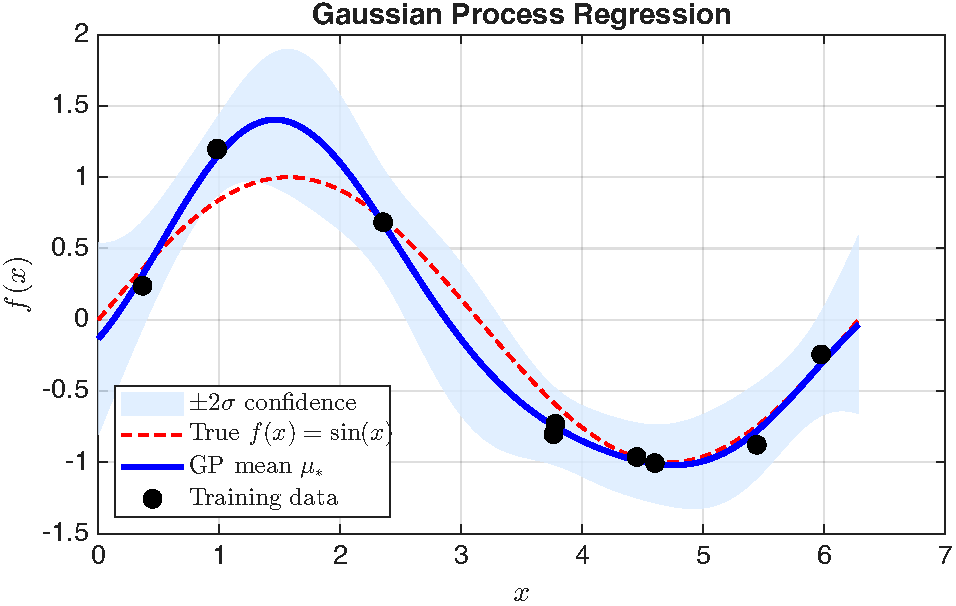
\includegraphics[width=0.85\textwidth]{Figures/fig_gp_regression.pdf}
	\caption{Gaussian Process regression on noisy observations of $f(x) = \sin(x)$. The GP mean interpolates the training data, and the 95\% confidence band widens away from data points, reflecting increasing prediction uncertainty. With 10 observations and a squared exponential kernel ($\sigma_f = 1$, $\ell = 1$), the GP captures the sinusoidal shape while honestly reporting its confidence.}
	\label{fig:gp_regression}
\end{figure}


\subsection{Learning Unknown Dynamics with GPs}
\label{sec:gp_dynamics}

Returning to the residual model~\eqref{eq:residual_model}, suppose we have collected $T$ state transitions from the real plant:
\[
\{(x_k, u_k, x_{k+1})\}_{k=0}^{T-1}
\]
The residual at each time step is:
\begin{equation}\label{eq:residual_data}
	r_k = x_{k+1} - Ax_k - Bu_k
\end{equation}
This is the part of the dynamics the nominal model fails to explain. Each $r_k$ is a noisy observation of $g(x_k, u_k)$.

For a system with $n$ states, $g$ maps $\mathbb{R}^{n+m}$ to $\mathbb{R}^n$. We fit \emph{one independent GP per state dimension}: the $i$th GP is trained on inputs $\{(x_k, u_k)\}$ and outputs $\{r_{k,i}\}$, where $r_{k,i}$ is the $i$th component of $r_k$.

After training, given a current state $x$ and input $u$, the GP provides:
\begin{align*}
	\text{Predicted next state:} \quad & \hat{x}_{k+1} = Ax_k + Bu_k + \mu_g(x_k, u_k) \\
	\text{Prediction uncertainty:} \quad & \Sigma_{k+1} = \text{diag}\bigl(\sigma_{g,1}^2(x_k, u_k), \ldots, \sigma_{g,n}^2(x_k, u_k)\bigr)
\end{align*}
where $\mu_g$ and $\Sigma_{k+1}$ are assembled from the individual GP predictions.

\begin{alertbox}{Computational Complexity}
	GP prediction requires solving a $T \times T$ linear system, which scales as $O(T^3)$. For small to moderate datasets ($T < 500$), this is fast. For larger datasets, sparse GP approximations using \emph{inducing points} reduce the cost to $O(TM^2)$, where $M \ll T$ is the number of inducing points. For the examples in these notes, exact GP inference is sufficient.
\end{alertbox}

Figure~\ref{fig:gp_residual} illustrates this process for the worked example in Section~\ref{sec:gpmpc_example}: the GP learns the unknown cubic drag $g(x) = -0.2\,x^3$ from 20 residual data points. The confidence band is narrow where data is concentrated and widens at the extremes.

\begin{figure}[ht]
	\centering
	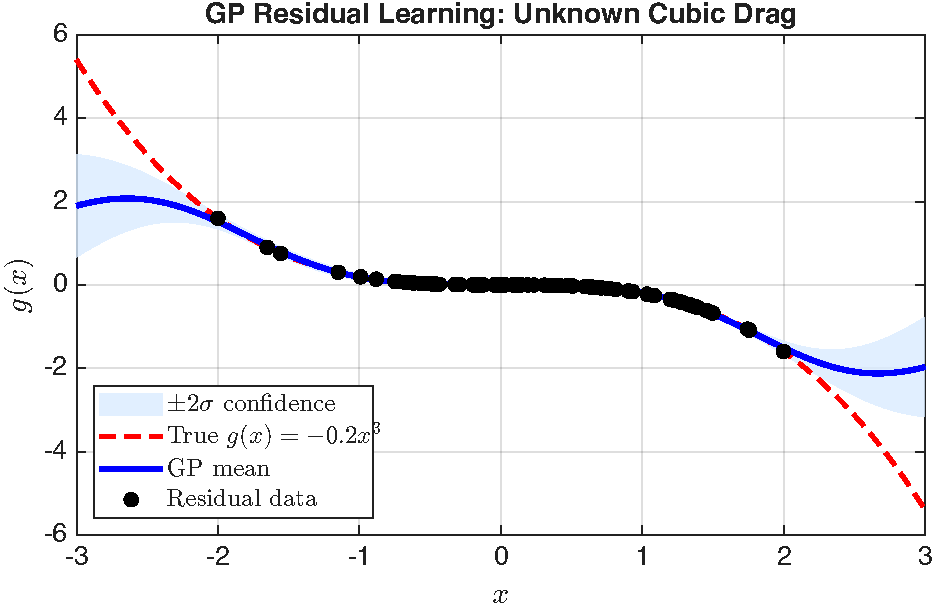
\includegraphics[width=0.85\textwidth]{Figures/fig_gp_residual.pdf}
	\caption{GP residual learning for the unknown cubic drag $g(x) = -0.2\,x^3$. The GP mean (blue) closely matches the true residual (red dashed) in the data-rich region $|x| \lesssim 2$, while the 95\% confidence band (shaded) widens outside this range. The black dots are the computed residuals $r_k = x_{k+1} - x_k - u_k$ from 20 exploratory data points.}
	\label{fig:gp_residual}
\end{figure}


\subsection{The GP-MPC Optimisation Problem}
\label{sec:gpmpc_formulation}

At each time step, the GP-enhanced model predicts the mean trajectory and the state-dependent uncertainty. This uncertainty is exploited through \emph{chance constraints}: instead of requiring that constraints hold with certainty (which would require worst-case reasoning as in Tube MPC), we require that they hold with a specified probability $1 - \delta$.

For each state dimension $i$ and each prediction step $k$, the state constraint $x_{k,i} \le x_{\max,i}$ becomes:
\begin{equation}\label{eq:chance_constraint}
	\Pr\bigl(x_{k,i} \le x_{\max,i}\bigr) \ge 1 - \delta
\end{equation}
For a \emph{single} prediction step, if the GP prediction is Gaussian, this is equivalent to a deterministic tightened constraint:
\begin{equation}\label{eq:tightened_chance}
	\boxed{\mu_{k,i} + \Phi^{-1}(1-\delta)\;\sigma_{k,i} \le x_{\max,i}}
\end{equation}
where $\Phi^{-1}$ is the inverse of the standard normal CDF (e.g.\ $\Phi^{-1}(0.95) \approx 1.645$ for a 95\% constraint, $\Phi^{-1}(0.975) \approx 1.96$ for 97.5\%).

\begin{alertbox}{Multi-Step Validity}
	The Gaussian tightening~\eqref{eq:tightened_chance} is exact at the first prediction step ($k=1$), because the one-step GP prediction is Gaussian by construction. For $k > 1$, the predicted state distribution is obtained by propagating through the nonlinear GP mean, which destroys the Gaussian structure. In practice, the formula is applied at every horizon step as a tractable \emph{approximation}---evaluating the GP variance at the current nominal trajectory rather than propagating uncertainty forward. This ``certainty-equivalent'' approach works well when the GP variance is small, but does not provide formal multi-step chance constraint guarantees.
\end{alertbox}

\begin{defnbox}{Chance Constraint Tightening via GP Variance}
	The GP variance $\sigma_{k,i}^2$ acts as a \emph{state-dependent safety margin}. In regions with little training data, $\sigma_{k,i}$ is large, and the constraint is tightened aggressively. In well-explored regions, $\sigma_{k,i}$ is small, and the constraint is barely tightened.
\end{defnbox}

\begin{notebox}{Connection to Tube MPC}
	Tube MPC (previous chapter) tightens constraints by a \emph{fixed} amount $\mathcal{E}$, determined by the worst-case disturbance bound $\mathcal{W}$. GP-MPC tightens constraints \emph{adaptively}: more where data is sparse (high variance), less where data is dense (low variance). As more data is collected, the GP variance shrinks everywhere, and the tightening approaches zero---the controller recovers the full feasible region.
\end{notebox}

The GP-MPC optimisation at time $t$ is:
\begin{equation}\label{eq:gpmpc_opt}
	\min_{u_0, \ldots, u_{N-1}} \; \sum_{k=0}^{N-1}\bigl(\mu_{x_k}^\top Q\,\mu_{x_k} + u_k^\top R\,u_k\bigr) + \mu_{x_N}^\top P\,\mu_{x_N}
\end{equation}
subject to:
\begin{align*}
	\text{Initialisation:} \quad & \mu_{x_0} = x(t) \\
	\text{Learned dynamics:} \quad & \mu_{x_{k+1}} = A\,\mu_{x_k} + B\,u_k + \mu_g(\mu_{x_k}, u_k) \\
	\text{Chance constraints:} \quad & \mu_{x_{k,i}} + \Phi^{-1}(1-\delta)\,\sigma_{x_{k,i}} \le x_{\max,i} \\
	& \mu_{x_{k,i}} - \Phi^{-1}(1-\delta)\,\sigma_{x_{k,i}} \ge x_{\min,i} \\
	\text{Actuator limits:} \quad & u_{\min} \le u_k \le u_{\max}
\end{align*}
for $k = 0, \ldots, N-1$ and $i = 1, \ldots, n$. The terminal cost $P$ is computed from the DARE applied to the nominal $(A, B)$.


\subsection{Worked Example: GP-MPC for a System with Unknown Nonlinearity}
\label{sec:gpmpc_example}

\begin{examplebox}{GP-MPC: Learning an Unknown Cubic Drag}
	\emph{System.} The true plant is a scalar system with a nonlinear drag term:
	\[
	x_{k+1} = x_k + u_k - 0.2\,x_k^3
	\]
	The cubic term $-0.2\,x_k^3$ is unknown to the controller.

	\emph{Nominal model.} The controller uses a pure integrator: $x_{k+1} = x_k + u_k$, i.e.\ $A = 1$, $B = 1$.

	\emph{Constraints.} $|u_k| \le 1$, $|x_k| \le 3$.

	\emph{Objective.} Regulate to the origin from $x_0 = 2.5$ with $Q = 1$, $R = 0.1$, $N = 10$.

	\solution

	\emph{Step 1: Data collection.} We excite the system with 20 random inputs from $u \sim \mathcal{U}(-1, 1)$ starting from $x_0 = 0$, and record the transitions.

	\emph{Step 2: Compute residuals.} For each transition, $r_k = x_{k+1} - x_k - u_k$. These residuals are noisy observations of $g(x_k) = -0.2\,x_k^3$.

	\emph{Step 3: Train GP.} Fit a GP with SE kernel to the residual data. The GP learns $g(x)$ along with pointwise confidence.

	\emph{Step 4: GP-MPC loop.} At each step:
	\begin{enumerate}[noitemsep]
		\item Query the GP at the current predicted states to obtain $\mu_g$ and $\sigma_g$.
		\item Formulate the MPC with tightened constraints: $\mu_{x_k} + 1.96\,\sigma_{x_k} \le 3$ and $\mu_{x_k} - 1.96\,\sigma_{x_k} \ge -3$.
		\item Solve the resulting NLP---or, more commonly, the QP approximation obtained by evaluating the GP at the current nominal trajectory (successive linearisation). Apply $u_0^*$, measure $x_{k+1}$, and optionally append the new data point to the GP training set.
	\end{enumerate}

\begin{lstlisting}[language=Matlab, caption={GP-MPC for a scalar system with unknown cubic drag.}]
% 1. True Plant and Nominal Model
A_nom = 1;  B_nom = 1;
f_true = @(x, u) x + u - 0.2*x^3;

% 2. Data Collection (random excitation)
rng(0);
T_data = 20;
x_data = zeros(T_data+1, 1);
u_data = 2*rand(T_data, 1) - 1;
for k = 1:T_data
    x_data(k+1) = f_true(x_data(k), u_data(k));
end
X_train = x_data(1:T_data);
r_train = x_data(2:T_data+1) - A_nom*x_data(1:T_data) ...
          - B_nom*u_data;

% 3. GP Training (SE kernel)
sf = 0.5;  ell = 1.0;  sn2 = 0.01;
kSE  = @(xa, xb) sf^2*exp(-0.5*(xa - xb').^2 / ell^2);
K_gp = kSE(X_train, X_train) + sn2*eye(T_data);
alpha_gp = K_gp \ r_train;

gp_mean = @(xs) kSE(xs, X_train) * alpha_gp;
gp_var  = @(xs) sf^2 - diag(kSE(xs, X_train) ...
                * (K_gp \ kSE(X_train, xs)));

% 4. GP-MPC Simulation
N = 10;  Q = 1;  R = 0.1;  P = dare(A_nom, B_nom, Q, R);
x_max = 3;  u_max = 1;  delta = 0.025;
kappa = norminv(1 - delta);  % 1.96 for 97.5%

T_sim  = 30;
x_hist = zeros(1, T_sim+1);  x_hist(1) = 2.5;
u_hist = zeros(1, T_sim);

for t = 1:T_sim
    x_now = x_hist(t);
    % Successive linearisation: evaluate GP at nominal trajectory
    x_nom = zeros(1, N+1);  x_nom(1) = x_now;
    mu_nom = zeros(1, N);  sig_nom = zeros(1, N);
    for k = 1:N
        mu_nom(k)  = gp_mean(x_nom(k));
        sig_nom(k) = sqrt(max(gp_var(x_nom(k)), 1e-6));
        x_nom(k+1) = A_nom*x_nom(k) + B_nom*0 + mu_nom(k);  % u=0 nominal
        % Simplification: a production implementation would use the previous MPC solution
    end
    % Build QP with GP evaluated at nominal (fixed, not decision vars)
    u_var = sdpvar(1, N);
    x_var = sdpvar(1, N+1);
    con = [x_var(1) == x_now];
    obj = 0;
    for k = 1:N
        con = [con, x_var(k+1) == A_nom*x_var(k) + B_nom*u_var(k) + mu_nom(k)];
        con = [con, -u_max <= u_var(k) <= u_max];
        con = [con, -x_max + kappa*sig_nom(k) <= x_var(k+1) <= x_max - kappa*sig_nom(k)];
        obj = obj + Q*x_var(k)^2 + R*u_var(k)^2;
    end
    obj = obj + P*x_var(N+1)^2;
    opts = sdpsettings('verbose', 0, 'solver', 'quadprog');
    optimize(con, obj, opts);
    u_hist(t)    = value(u_var(1));
    x_hist(t+1)  = f_true(x_hist(t), u_hist(t));
end
\end{lstlisting}

\begin{alertbox}{Computational note}
The code above calls \texttt{optimize} inside the loop, rebuilding the YALMIP problem at every time step.  This is acceptable for a small demonstration but very slow in practice.  For real applications, reformulate the problem using YALMIP's \texttt{optimizer} object with the GP-derived tightening values as additional parameters.
\end{alertbox}

\begin{lstlisting}[language=Matlab]

% 5. Plot Results
figure;
subplot(2,1,1); stairs(0:T_sim-1, u_hist, 'b', 'LineWidth', 2);
yline(u_max, 'r--', 'LineWidth', 1.5); yline(-u_max, 'r--', 'LineWidth', 1.5);
ylabel('u_k'); title('GP-MPC: Control Input'); grid on;
subplot(2,1,2); plot(0:T_sim, x_hist, 'b', 'LineWidth', 2);
yline(x_max, 'r--', 'LineWidth', 1.5); yline(-x_max, 'r--', 'LineWidth', 1.5);
ylabel('x_k'); xlabel('Time step k'); title('GP-MPC: State'); grid on;
\end{lstlisting}
\end{examplebox}

\begin{summarybox}{GP-MPC Design Recipe}
	\begin{enumerate}
		\item Collect trajectory data from the real system under exploratory excitation.
		\item Compute residuals $r_k = x_{k+1} - Ax_k - Bu_k$ and train a GP (one per state dimension).
		\item At each MPC step, query the GP for the predicted residual mean $\mu_g$ and variance $\sigma_g^2$.
		\item Tighten the state constraints using~\eqref{eq:tightened_chance}: $\mu_{k,i} + \kappa\,\sigma_{k,i} \le x_{\max,i}$, where $\kappa = \Phi^{-1}(1-\delta)$.
		\item Solve the resulting optimisation (an NLP in general; a QP if the GP is evaluated at the nominal trajectory). Apply $u_0^*$ and optionally update the GP with the new measurement.
	\end{enumerate}
\end{summarybox}

The closed-loop result of the GP-MPC controller is shown in Figure~\ref{fig:gpmpc_simulation}. Compared to the nominal controller (which ignores the cubic drag), GP-MPC achieves faster regulation and avoids the oscillatory behaviour caused by model mismatch.

\begin{figure}[ht]
	\centering
	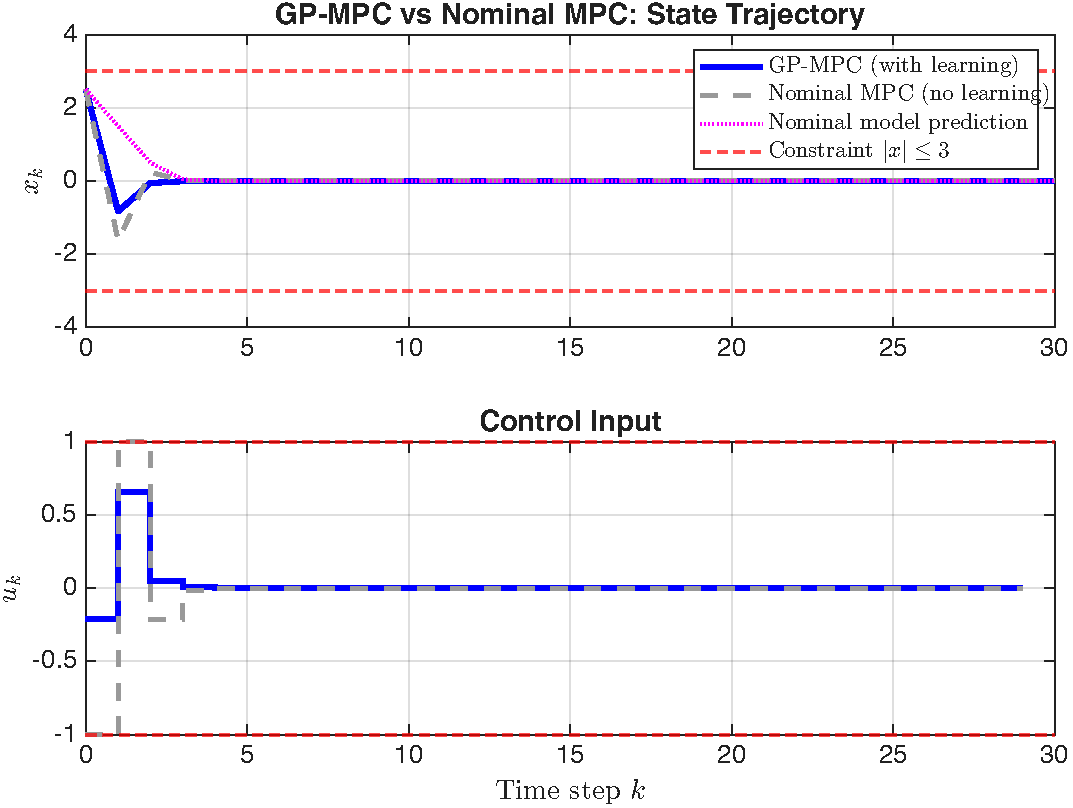
\includegraphics[width=0.88\textwidth]{Figures/fig_gpmpc_simulation.pdf}
	\caption{GP-MPC closed-loop simulation for the scalar system with unknown cubic drag. Top: state trajectory. The GP-MPC controller (blue) drives the state to the origin smoothly, while the nominal controller (grey dashed) exhibits slower convergence due to unmodelled dynamics. Bottom: control input. Both controllers respect the actuator limits $|u_k| \le 1$. The red dashed lines indicate the constraint boundaries.}
	\label{fig:gpmpc_simulation}
\end{figure}

Figure~\ref{fig:gpmpc_architecture} shows the GP-MPC control architecture as a block diagram. The GP model sits alongside the nominal model and feeds both the predicted mean and the predicted variance into the MPC optimisation.

\begin{figure}[ht]
	\centering
	\begin{tikzpicture}[
		>=Stealth,
		node distance=1.0cm and 1.6cm,
		block/.style={draw, rounded corners=3pt, fill=blue!8,
			minimum width=2.8cm, minimum height=1.0cm, align=center, font=\small},
		blockgp/.style={draw, rounded corners=3pt, fill=orange!15,
			minimum width=2.8cm, minimum height=1.0cm, align=center, font=\small},
		blockplant/.style={draw, rounded corners=3pt, fill=green!10,
			minimum width=2.4cm, minimum height=1.0cm, align=center, font=\small},
		sum/.style={draw, circle, minimum size=0.5cm, inner sep=0pt, font=\small},
		arr/.style={->, thick},
	]
		% MPC block
		\node[block] (mpc) {MPC Optimiser\\{\scriptsize (NLP solver)}};

		% Plant
		\node[blockplant, right=3.5cm of mpc] (plant) {True Plant\\$x_{k+1} = f(x_k, u_k)$};

		% GP block
		\node[blockgp, below=2.0cm of mpc] (gp) {GP Model\\$\mu_g(x,u),\; \sigma_g^2(x,u)$};

		% Nominal model
		\node[block, below=2.1cm of plant] (nom) {Nominal Model\\$Ax_k + Bu_k$};

		% Arrows
		\draw[arr] (mpc.east) -- node[above, font=\small] {$u_k^*$} (plant.west);
		\draw[arr] (plant.east) -- ++(1.0,0) node[above left, font=\small] {$x_{k+1}$} |- (nom.east);
		\draw[arr] (nom.west) -- node[above, font=\small] {$r_k$} (gp.east);
		\draw[arr] (gp.north) -- node[left, font=\small] {$\mu_g$, $\sigma_g^2$} (mpc.south);

		% Feedback: x_k to MPC
		\draw[arr] (plant.north) -- ++(0,1.0) -| node[above, pos=0.25, font=\small] {$x_k$ (measured)} (mpc.north);

		% Data collection annotation
		\node[right=1.0cm of nom, font=\scriptsize\itshape, text=gray] (ann) {residual data};
		\draw[->, gray, dashed] (plant.east) ++(1.0,0) |- (ann.east);
	\end{tikzpicture}
	\caption{GP-MPC architecture. At each time step, the measured state $x_k$ is used to query the GP model, which returns the predicted residual mean $\mu_g$ and variance $\sigma_g^2$. These are incorporated into the MPC optimisation as a dynamics correction and as state-dependent constraint tightening, respectively. The residual data $r_k = x_{k+1} - Ax_k - Bu_k$ can optionally be appended to the GP training set for online learning.}
	\label{fig:gpmpc_architecture}
\end{figure}


%% ============================================================
%%  SECTION 3: KOOPMAN OPERATOR AND DATA-DRIVEN LINEAR MODELS
%% ============================================================
\section{Koopman Operator and Data-Driven Linear Models}
\label{sec:koopman}

The GP-MPC approach learns a nonlinear correction to a known model. The Koopman approach takes a fundamentally different route: it transforms the entire nonlinear system into a \emph{linear} one by working in a higher-dimensional space. Once the system is linear, the standard MPC machinery from Chapter~7---quadratic cost, linear constraints, QP solver---applies directly.

\subsection{The Koopman Operator}
\label{sec:koopman_theory}

Consider an autonomous nonlinear system:
\[
x_{k+1} = f(x_k), \qquad x_k \in \mathbb{R}^n
\]
The state evolves in $\mathbb{R}^n$ according to the possibly complicated function $f$. Instead of tracking the state directly, consider tracking \emph{functions of the state}.

An \emph{observable} is any scalar function $\psi \colon \mathbb{R}^n \to \mathbb{R}$. For instance, $\psi(x) = x_1^2 + x_2$ is an observable. If we know $x_k$, we can compute $\psi(x_k)$. One time step later, $\psi$ takes the value $\psi(x_{k+1}) = \psi(f(x_k))$.

\begin{defnbox}{Definition: The Koopman Operator}
	The \emph{Koopman operator} $\mathcal{K}$ acts on observables:
	\[
	(\mathcal{K}\psi)(x) = \psi\bigl(f(x)\bigr)
	\]
	It advances any observable one time step forward along the trajectories of $f$. The crucial property is that $\mathcal{K}$ is \emph{linear}: $\mathcal{K}(\alpha\psi_1 + \beta\psi_2) = \alpha\,\mathcal{K}\psi_1 + \beta\,\mathcal{K}\psi_2$, even when $f$ is nonlinear. The trade-off is that $\mathcal{K}$ acts on a space of \emph{functions}, which is infinite-dimensional.
\end{defnbox}

In other words, nonlinear dynamics of states become \emph{linear dynamics of observables}. If we could find a finite set of observables closed under the action of $\mathcal{K}$, we would have an exact finite-dimensional linear representation of the nonlinear system. For most nonlinear systems, no such finite set exists---but a well-chosen finite dictionary can still produce an accurate approximation.

\subsubsection*{Finite-Dimensional Approximation}

In practice, we choose a \emph{dictionary} of $p$ observables:
\[
\Psi(x) = \begin{bmatrix} \psi_1(x) \\ \psi_2(x) \\ \vdots \\ \psi_p(x) \end{bmatrix} \in \mathbb{R}^p
\]
Common choices include monomials ($x_1$, $x_2$, $x_1^2$, $x_1 x_2$, $x_2^2$, \ldots), radial basis functions, or trigonometric functions. The \emph{lifted state} is $z_k = \Psi(x_k) \in \mathbb{R}^p$, with $p \ge n$. The first $n$ entries are typically chosen to be the original states: $\psi_i(x) = x_i$ for $i = 1, \ldots, n$.

We then seek a matrix $K_d \in \mathbb{R}^{p \times p}$ (we write $K_d$ to distinguish it from the feedback gain $K$ used elsewhere in these notes) such that:
\begin{equation}\label{eq:koopman_approx}
	z_{k+1} = \Psi(x_{k+1}) \approx K_d\,z_k = K_d\,\Psi(x_k)
\end{equation}
This is a \emph{linear} dynamical system in the lifted coordinates $z_k$. The nonlinearity of $f$ is absorbed into the choice of dictionary $\Psi$.

\begin{alertbox}{Dictionary Choice}
	The quality of the approximation~\eqref{eq:koopman_approx} depends entirely on the dictionary $\Psi$. A poor dictionary produces a poor linear model. Common strategies:
	\begin{itemize}[noitemsep]
		\item \emph{Monomials} up to a chosen degree (simple, intuitive, but the number of terms grows combinatorially).
		\item \emph{Radial basis functions} centred at representative states.
		\item \emph{Domain knowledge}: if the nonlinearity involves $x^3$, include $x^3$ in the dictionary.
	\end{itemize}
	There is no universal recipe; choosing a good dictionary remains an open research question.
\end{alertbox}


\subsection{Extended Dynamic Mode Decomposition (EDMD)}
\label{sec:edmd}

EDMD is the standard method for computing the Koopman approximation from data. For a system with control inputs, the dynamics are $x_{k+1} = f(x_k, u_k)$, and the lifted linear model becomes:
\begin{equation}\label{eq:koopman_controlled}
	z_{k+1} \approx A_K\,z_k + B_K\,u_k
\end{equation}

\subsubsection*{The Algorithm}

Collect a trajectory of $T$ state transitions:
\[
\{(x_0, u_0, x_1),\; (x_1, u_1, x_2),\; \ldots,\; (x_{T-2}, u_{T-2}, x_{T-1})\}
\]
Apply the dictionary $\Psi$ to each state:
\begin{align*}
	Z &= \bigl[\Psi(x_0) \;\; \Psi(x_1) \;\; \cdots \;\; \Psi(x_{T-2})\bigr] \in \mathbb{R}^{p \times (T-1)} \\
	Z' &= \bigl[\Psi(x_1) \;\; \Psi(x_2) \;\; \cdots \;\; \Psi(x_{T-1})\bigr] \in \mathbb{R}^{p \times (T-1)} \\
	U &= \bigl[u_0 \;\; u_1 \;\; \cdots \;\; u_{T-2}\bigr] \in \mathbb{R}^{m \times (T-1)}
\end{align*}

The matrices $A_K$ and $B_K$ are found by solving the least-squares problem:
\begin{equation}\label{eq:edmd_ls}
	\bigl[A_K \;\; B_K\bigr] = Z' \begin{bmatrix} Z \\ U \end{bmatrix}^\dagger
\end{equation}
where $\dagger$ denotes the Moore--Penrose pseudoinverse. This minimises $\sum_{k} \|\Psi(x_{k+1}) - A_K\Psi(x_k) - B_K u_k\|^2$.

\begin{examplebox}{Hand-Worked EDMD for a Scalar Nonlinear System}
	\emph{System.} $x_{k+1} = 0.9\,x_k + 0.1\,x_k^2 + u_k$.

	\emph{Dictionary.} $\Psi(x) = [x, \; x^2]^\top$ (two lifted states, $p = 2$).

	We collect 5 transitions from $x_0 = 1$ with inputs $u = [0.1,\; -0.2,\; 0.3,\; -0.1,\; 0.0]$:
	\[
	\begin{array}{c|c|c}
		k & x_k & u_k \\ \hline
		0 & 1.000 & 0.100 \\
		1 & 1.100 & -0.200 \\
		2 & 0.911 & 0.300 \\
		3 & 1.203 & -0.100 \\
		4 & 1.127 & 0.000
	\end{array}
	\]
	where $x_1 = 0.9(1) + 0.1(1)^2 + 0.1 = 1.1$, etc.

	\solution

	\emph{Step 1: Lift the data.}
	\[
	Z = \begin{bmatrix} 1.000 & 1.100 & 0.911 & 1.203 \\ 1.000 & 1.210 & 0.830 & 1.447 \end{bmatrix}, \quad
	Z' = \begin{bmatrix} 1.100 & 0.911 & 1.203 & 1.127 \\ 1.210 & 0.830 & 1.447 & 1.270 \end{bmatrix}
	\]
	\[
	U = \begin{bmatrix} 0.1 & -0.2 & 0.3 & -0.1 \end{bmatrix}
	\]

	\emph{Step 2: Solve.} Form the stacked matrix $\Omega = [Z;\; U] \in \mathbb{R}^{3 \times 4}$ and compute:
	\[
	[A_K \;\; B_K] = Z'\,\Omega^\dagger
	\]
	This yields $A_K \in \mathbb{R}^{2 \times 2}$ and $B_K \in \mathbb{R}^{2 \times 1}$. The resulting $A_K$ captures both the linear and quadratic dynamics in a single linear system.

	\emph{Step 3: Verify.} At $x = 1.5$ with $u = 0$:
	\begin{itemize}[noitemsep]
		\item True: $x^+ = 0.9(1.5) + 0.1(1.5)^2 = 1.575$
		\item Koopman: $z^+ = A_K [1.5,\; 2.25]^\top + B_K \cdot 0$, then extract the first component.
	\end{itemize}
	The predictions should be close, confirming the dictionary captures the quadratic nonlinearity.
\end{examplebox}

The following MATLAB code performs EDMD identification and compares the Koopman prediction to the true dynamics.

\begin{lstlisting}[language=Matlab, caption={EDMD identification for a scalar nonlinear system.}]
% 1. True Nonlinear Plant
f_true = @(x, u) 0.9*x + 0.1*x.^2 + u;

% 2. Data Collection
rng(1);
T = 50;
x_data = zeros(T+1, 1);  x_data(1) = 0;
u_data = 0.5*randn(T, 1);
for k = 1:T
    x_data(k+1) = f_true(x_data(k), u_data(k));
end

% 3. Dictionary: Psi(x) = [x; x^2]
Psi = @(x) [x; x.^2];
p = 2;  % lifted dimension

Z  = zeros(p, T);  Zp = zeros(p, T);
for k = 1:T
    Z(:,k)  = Psi(x_data(k));
    Zp(:,k) = Psi(x_data(k+1));
end
U = u_data(1:T)';

% 4. EDMD: Solve [A_K, B_K] = Zp * [Z; U]'
Omega = [Z; U];
AB = Zp * pinv(Omega);
A_K = AB(:, 1:p);
B_K = AB(:, p+1:end);

% 5. Verify: One-Step Prediction
x_test = linspace(-2, 2, 100);
x_true = f_true(x_test, 0);
x_koop = zeros(1, 100);
for i = 1:100
    z_next = A_K * Psi(x_test(i)) + B_K * 0;
    x_koop(i) = z_next(1);  % extract first component
end

figure; plot(x_test, x_true, 'r-', 'LineWidth', 2); hold on;
plot(x_test, x_koop, 'b--', 'LineWidth', 2);
xlabel('x_k'); ylabel('x_{k+1}');
legend('True dynamics', 'Koopman (EDMD)');
title('EDMD One-Step Prediction (u = 0)'); grid on;
\end{lstlisting}

Figure~\ref{fig:edmd_prediction} compares the Koopman predictor to the true dynamics. The Koopman model (blue dashed) captures the quadratic nonlinearity accurately, while the linearisation about the origin (grey dotted) diverges significantly for $|x| > 1$.

\begin{figure}[ht]
	\centering
	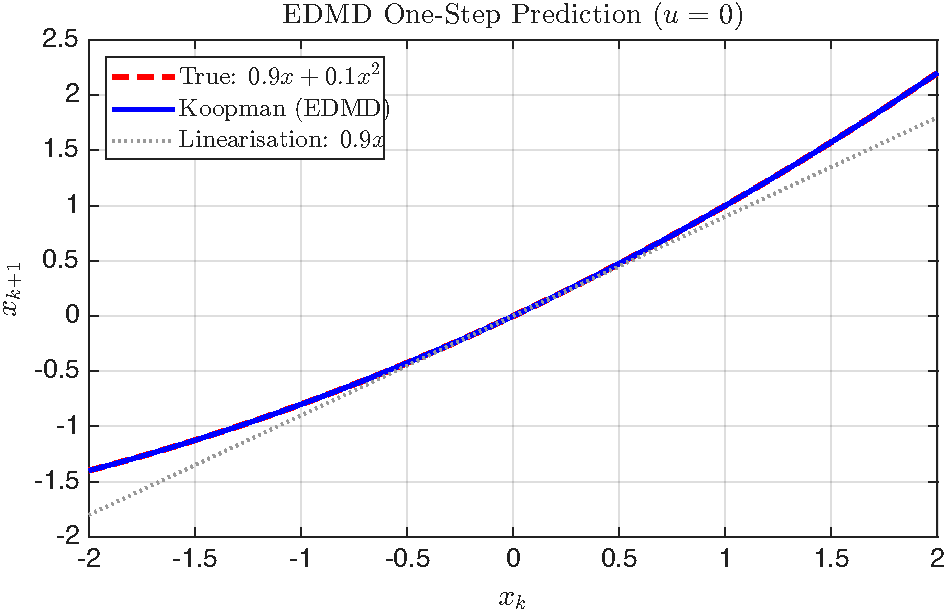
\includegraphics[width=0.82\textwidth]{Figures/fig_edmd_prediction.pdf}
	\caption{EDMD one-step prediction comparison for the scalar system $x_{k+1} = 0.9\,x_k + 0.1\,x_k^2$ (with $u = 0$). The Koopman model identified from 50 data points with dictionary $\Psi(x) = [x,\; x^2]^\top$ closely matches the true nonlinear dynamics (red dashed) --- indeed the two curves overlap almost perfectly, confirming that the dictionary $[x,\; x^2]$ captures the dynamics exactly. The linearisation about the origin (grey dotted, $x_{k+1} \approx 0.9\,x_k$) captures only the linear part and becomes inaccurate away from the origin.}
	\label{fig:edmd_prediction}
\end{figure}


\subsection{Koopman MPC}
\label{sec:koopman_mpc}

With the identified matrices $(A_K, B_K)$, we formulate a standard linear MPC in the lifted coordinates. The optimisation is identical in structure to the one in Chapter~7---it is a QP.

Let $C_x \in \mathbb{R}^{n \times p}$ be the matrix that extracts the original states from the lifted state, i.e.\ $x_k = C_x\,z_k$. Since we chose $\psi_i(x) = x_i$ for $i = 1, \ldots, n$, we simply have $C_x = [I_n \;\; 0]$.

The cost matrices in lifted space are:
\[
\tilde{Q} = C_x^\top Q\,C_x
\]
The terminal cost $\tilde{P}$ is obtained by solving the DARE for the lifted system: $\tilde{P}$ is the stabilising solution of the discrete algebraic Riccati equation with $(A_K, B_K, \tilde{Q}, R)$.

The Koopman MPC problem at time $t$ is:
\begin{equation}\label{eq:koopman_mpc}
	\min_{u_0, \ldots, u_{N-1}} \; \sum_{k=0}^{N-1}\bigl(z_k^\top \tilde{Q}\,z_k + u_k^\top R\,u_k\bigr) + z_N^\top \tilde{P}\,z_N
\end{equation}
subject to:
\begin{align*}
	\text{Initialisation:} \quad & z_0 = \Psi\bigl(x(t)\bigr) \\
	\text{Lifted dynamics:} \quad & z_{k+1} = A_K\,z_k + B_K\,u_k \\
	\text{State constraints:} \quad & x_{\min} \le C_x\,z_k \le x_{\max} \\
	\text{Actuator limits:} \quad & u_{\min} \le u_k \le u_{\max}
\end{align*}

\begin{notebox}{Reusing the Linear MPC Machinery}
	The Koopman MPC problem~\eqref{eq:koopman_mpc} is a standard QP. The YALMIP implementation from Chapter~7 can be reused with minimal changes: replace $A$ with $A_K$, $B$ with $B_K$, $x_k$ with $z_k$, and adjust the cost matrices. The stability theory from Chapter~7---terminal cost, terminal set, recursive feasibility---applies to the \emph{identified Koopman model}. Whether these guarantees transfer to the true nonlinear system depends on the accuracy of the dictionary approximation: a poor dictionary may produce a model whose predictions diverge from the true dynamics, invalidating the stability argument.
\end{notebox}


\subsection{Worked Example: Koopman MPC for a Duffing-Type Oscillator}
\label{sec:koopman_example}

\begin{examplebox}{Koopman MPC for a Nonlinear Oscillator}
	\emph{System.} A Duffing oscillator discretised with RK4 at sampling time $T_s = 0.2$:
	\begin{align*}
		\dot{x}_1 &= x_2, \qquad
		\dot{x}_2 = -x_1 - 3\,x_1^3 - 0.3\,x_2 + u
	\end{align*}
	The strong cubic stiffness ($\beta = 3$) makes this system heavily nonlinear for $|x_1| > 1$.

	\emph{Dictionary.} $\Psi(x) = [x_1,\; x_2,\; x_1^2,\; x_2^2,\; x_1 x_2]^\top$ ($p = 5$ lifted states).

	\emph{Constraints.} $|u_k| \le 2$, $|x_{1,k}| \le 5$ (soft).

	\emph{Objective.} Regulate from $x_0 = [3;\; 0]$ to the origin with $Q = \text{diag}(10, 1)$, $R = 0.1$, $N = 10$.

	\solution

	We collect 1440 data points from 12 diverse initial conditions with random excitation, identify $(A_K, B_K)$ via EDMD, and compare Koopman MPC against linearised MPC using YALMIP. Both controllers use identical MPC formulations; only the prediction model differs.

\begin{lstlisting}[language=Matlab, caption={Koopman MPC vs Linearised MPC for a Duffing oscillator (RK4).}]
% 1. True Nonlinear Plant (RK4 discretisation)
Ts = 0.2;  alpha = 1;  beta = 3;  delta = 0.3;
f_cont = @(x,u) [x(2); -alpha*x(1)-beta*x(1)^3-delta*x(2)+u];
rk4 = @(x,u) rk4_step(f_cont, x, u, Ts);

% Linearisation at origin (numerical Jacobian of RK4 map)
eps_j = 1e-6;
A_lin = zeros(2);
for j = 1:2
    xp = zeros(2,1); xp(j) = eps_j;
    xm = zeros(2,1); xm(j) = -eps_j;
    A_lin(:,j) = (rk4(xp,0)-rk4(xm,0))/(2*eps_j);
end
B_lin = (rk4(zeros(2,1),eps_j)-rk4(zeros(2,1),-eps_j))/(2*eps_j);

% 2. Data Collection (diverse ICs for broad coverage)
rng(42);  nx = 2;
ics = [2 0;-2 0;0 2;0 -2;1.5 1;-1 -1.5;2.5 -1;-2.5 1;
       1 1;-1 1;3 0;-3 0]';
X_all=[];  Xp_all=[];  U_all=[];
for b = 1:size(ics,2)
    x = ics(:,b);
    for k = 1:120
        u = 2.5*randn;  xn = rk4(x, u);
        if any(abs(xn)>10), xn = 0.3*randn(2,1); end
        X_all=[X_all,x]; Xp_all=[Xp_all,xn]; U_all=[U_all,u];
        x = xn;
    end
end

% 3. EDMD Identification
Psi = @(x) [x(1);x(2);x(1)^2;x(2)^2;x(1)*x(2)];
p = 5;  Z = zeros(p,size(X_all,2));  Zp = Z;
for k = 1:size(X_all,2)
    Z(:,k) = Psi(X_all(:,k));  Zp(:,k) = Psi(Xp_all(:,k));
end
AB = Zp * pinv([Z; U_all]);
A_K = AB(:,1:p);  B_K = AB(:,p+1:end);
Cx = [eye(nx), zeros(nx,p-nx)];

% 4. Build Koopman MPC and Linearised MPC (both via YALMIP)
Q = diag([10,1]);  R = 0.1;  N = 10;
u_max = 2;  x1_max = 5;  lam_s = 1e4;
opts = sdpsettings('verbose',0,'solver','quadprog');
Q_lift = Cx'*Q*Cx;

% Koopman MPC
z_par = sdpvar(p,1);  uK = sdpvar(N,1);  sK = sdpvar(N,1);
zp = cell(N+1,1);  zp{1} = z_par;
for k = 1:N, zp{k+1} = A_K*zp{k} + B_K*uK(k); end
objK = 0;  conK = [sK >= 0];
for k = 1:N
    xk = Cx*zp{k+1};
    objK = objK + xk'*Q*xk + R*uK(k)^2 + lam_s*sK(k)^2;
    conK = [conK, -u_max<=uK(k)<=u_max];
    conK = [conK, -x1_max-sK(k)<=xk(1)<=x1_max+sK(k)];
end
koopman_ctrl = optimizer(conK, objK, opts, z_par, uK(1));

% Linearised MPC (same structure, different model)
x_par = sdpvar(nx,1);  uL = sdpvar(N,1);  sL = sdpvar(N,1);
xp = cell(N+1,1);  xp{1} = x_par;
for k = 1:N, xp{k+1} = A_lin*xp{k} + B_lin*uL(k); end
objL = 0;  conL = [sL >= 0];
for k = 1:N
    objL = objL + xp{k+1}'*Q*xp{k+1} + R*uL(k)^2 + lam_s*sL(k)^2;
    conL = [conL, -u_max<=uL(k)<=u_max];
    conL = [conL, -x1_max-sL(k)<=xp{k+1}(1)<=x1_max+sL(k)];
end
linear_ctrl = optimizer(conL, objL, opts, x_par, uL(1));

% 5. Closed-Loop Simulation
T_sim = 60;  x0 = [3; 0];
xK = zeros(nx,T_sim+1); xK(:,1) = x0; uK_h = zeros(1,T_sim);
xL = zeros(nx,T_sim+1); xL(:,1) = x0; uL_h = zeros(1,T_sim);
for t = 1:T_sim
    [uopt,~] = koopman_ctrl(Psi(xK(:,t)));
    uK_h(t) = max(-u_max, min(u_max, full(uopt)));
    xK(:,t+1) = rk4(xK(:,t), uK_h(t));
    [uopt,~] = linear_ctrl(xL(:,t));
    uL_h(t) = max(-u_max, min(u_max, full(uopt)));
    xL(:,t+1) = rk4(xL(:,t), uL_h(t));
end

% Helper: RK4 step
function xn = rk4_step(f, x, u, h)
    k1=f(x,u); k2=f(x+0.5*h*k1,u);
    k3=f(x+0.5*h*k2,u); k4=f(x+h*k3,u);
    xn = x + (h/6)*(k1+2*k2+2*k3+k4);
end
\end{lstlisting}
\end{examplebox}

Figure~\ref{fig:koopman_mpc} compares the two controllers in closed loop. The key difference is visible from the very first time step: at $x_0 = [3;\; 0]$, the linearised controller applies maximum negative input ($u = -2$) because it does not anticipate the strong cubic restoring force. The Koopman controller, which captures this nonlinearity through the lifted dictionary, applies a much smaller input ($u \approx 0.2$) --- it knows the cubic stiffness will pull the state back. Over the full trajectory, Koopman MPC achieves approximately 11\% lower cost and settles roughly 10 steps faster.

\begin{figure}[ht]
	\centering
	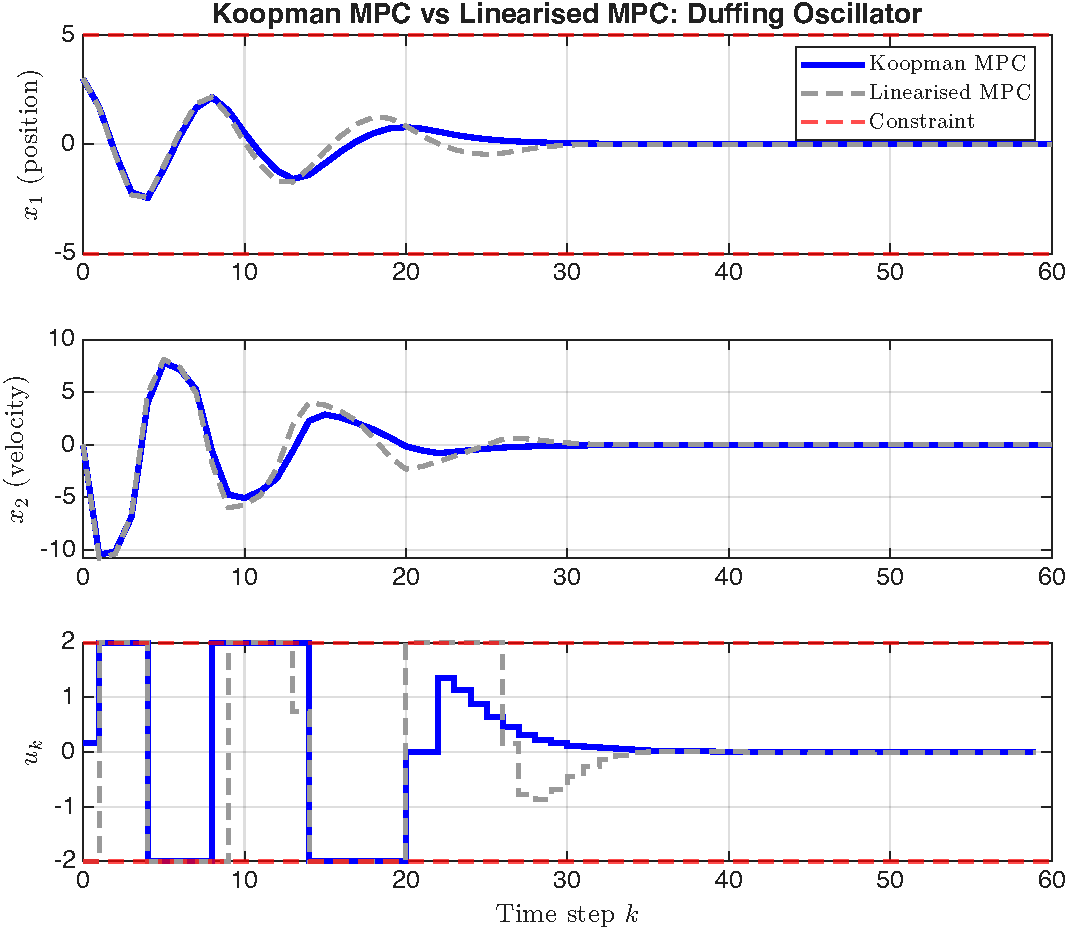
\includegraphics[width=0.88\textwidth]{Figures/fig_koopman_mpc.pdf}
	\caption{Koopman MPC vs linearised MPC for the Duffing oscillator ($\beta = 3$, RK4, $T_s = 0.2$). Top: position $x_1$. Middle: velocity $x_2$. Bottom: control input $u_k$. At $x_0 = [3;\;0]$, the linearised controller (grey dashed) applies maximum effort because it cannot predict the cubic restoring force, leading to larger oscillations. The Koopman controller (blue solid) uses the EDMD-identified lifted model with dictionary $\Psi(x) = [x_1,\; x_2,\; x_1^2,\; x_2^2,\; x_1 x_2]^\top$, exploits the nonlinearity, and settles faster with lower cost.}
	\label{fig:koopman_mpc}
\end{figure}


%% ============================================================
%%  SECTION 4: DATA-ENABLED PREDICTIVE CONTROL (DeePC)
%% ============================================================
\section{Data-Enabled Predictive Control (DeePC)}
\label{sec:deepc}

GP-MPC learns a model correction; Koopman MPC learns a linear representation. Both require an intermediate modelling step. DeePC eliminates this step entirely: raw input--output measurements enter the MPC optimisation directly. The data \emph{is} the model.

The theoretical foundation is \emph{Willems' Fundamental Lemma}, which guarantees that sufficiently rich data from a linear time-invariant (LTI) system captures \emph{all possible} system behaviours.

\subsection{Persistently Exciting Data}
\label{sec:pe}

For data to fully represent a system, the input signal used to collect it must be sufficiently ``rich.'' A constant input reveals nothing about the system's dynamics; a random signal, by contrast, excites all modes.

\begin{defnbox}{Definition: Hankel Matrix}
	Given a signal $\{u_0, u_1, \ldots, u_{T-1}\}$ of length $T$ and a depth $L \le T$, the \emph{Hankel matrix} of depth $L$ is:
	\[
	\mathcal{H}_L(u) = \begin{bmatrix}
		u_0     & u_1     & \cdots & u_{T-L} \\
		u_1     & u_2     & \cdots & u_{T-L+1} \\
		\vdots  &         & \ddots & \vdots \\
		u_{L-1} & u_L     & \cdots & u_{T-1}
	\end{bmatrix} \in \mathbb{R}^{mL \times (T-L+1)}
	\]
	where $m$ is the dimension of $u_k$. Each column is a consecutive length-$L$ window of the signal.
\end{defnbox}

\begin{defnbox}{Definition: Persistence of Excitation}
	A signal $\{u_0, \ldots, u_{T-1}\}$ is \emph{persistently exciting} (PE) of order $L$ if the Hankel matrix $\mathcal{H}_L(u)$ has \emph{full row rank}, i.e.\ $\text{rank}\bigl(\mathcal{H}_L(u)\bigr) = mL$.

	A random signal (e.g.\ $u_k \sim \mathcal{N}(0, \sigma^2)$) is PE of any order with probability one, provided $T$ is large enough. A constant or periodic signal is not PE of high order.
\end{defnbox}

\subsection{Willems' Fundamental Lemma}
\label{sec:willems}

We now state the central result that underpins DeePC.

Let $(u^d, y^d) = \{(u_0^d, y_0^d), (u_1^d, y_1^d), \ldots, (u_{T-1}^d, y_{T-1}^d)\}$ be a single input--output trajectory of length $T$ collected from an LTI system of order $n$ (i.e.\ the system has $n$ states). Construct the stacked Hankel matrix:
\[
\mathcal{H}_L\!\binom{u^d}{y^d} = \begin{bmatrix} \mathcal{H}_L(u^d) \\ \mathcal{H}_L(y^d) \end{bmatrix}
\]

\begin{defnbox}{Willems' Fundamental Lemma~\cite{Willems2005}}
	Assume the LTI system is \emph{controllable} (i.e.\ the pair $(A, B)$ has full rank controllability matrix). If $u^d$ is persistently exciting of order $L + n$, then $(u, y)$ is a valid length-$L$ input--output trajectory of the system \emph{if and only if} there exists a vector $g \in \mathbb{R}^{T-L+1}$ such that:
	\begin{equation}\label{eq:fundamental_lemma}
		\begin{bmatrix} \mathcal{H}_L(u^d) \\ \mathcal{H}_L(y^d) \end{bmatrix} g = \begin{bmatrix} u \\ y \end{bmatrix}
	\end{equation}
\end{defnbox}

The PE order is $L + n$ rather than $L$ alone because the extra $n$ rows are needed to span the $n$-dimensional initial state space on top of the $L$-step trajectory space. Controllability ensures that all modes can be reached by the input.

In plain language: the columns of the stacked Hankel matrix span every possible length-$L$ trajectory the system can produce. To generate any specific trajectory $(u, y)$, we find a linear combination $g$ of the data columns. The vector $g$ is not a physical quantity---it is simply the ``recipe'' for combining stored data windows.

\begin{examplebox}{Verifying the Fundamental Lemma}
	\emph{System.} A first-order system: $x_{k+1} = 0.8\,x_k + u_k$, $y_k = x_k$, so $n = 1$.

	We collect $T = 10$ data points with input $u^d = [0.5,\; -1.2,\; 0.3,\; 0.8,\; -0.6,\; 1.1,\; -0.4,\; 0.7,\; -0.9,\; 0.2]$ starting from $x_0 = 0$. The corresponding output $y^d$ is computed from the recursion.

	\solution

	Choose $L = 3$. The PE condition requires $u^d$ to be PE of order $L + n = 4$. The Hankel matrix $\mathcal{H}_4(u^d) \in \mathbb{R}^{4 \times 7}$ must have rank~4. For a random-like input with $T = 10$, this is easily satisfied.

	Construct the stacked Hankel matrix $\mathcal{H}_3\binom{u^d}{y^d} \in \mathbb{R}^{6 \times 8}$.

	Now pick any valid 3-step trajectory. For instance, start from $x_0 = 1$ with $u = [0.5,\; -0.3,\; 0.1]$. Compute $y = [1.0,\; 1.3,\; 0.74]$ from the recursion. Then find $g$ such that~\eqref{eq:fundamental_lemma} holds by solving the (overdetermined) linear system. If the data is PE, a solution $g$ exists.

\begin{lstlisting}[language=Matlab, caption={Verifying Willems' Fundamental Lemma.}]
% 1. System
a = 0.8;  b = 1;  n = 1;

% 2. Data Collection
ud = [0.5, -1.2, 0.3, 0.8, -0.6, 1.1, -0.4, 0.7, -0.9, 0.2];
T = length(ud);
xd = zeros(1, T+1);  xd(1) = 0;
for k = 1:T
    xd(k+1) = a*xd(k) + b*ud(k);
end
yd = xd(1:T);  % y_k = x_k

% 3. Build Hankel Matrices (depth L = 3)
L = 3;
Hu = zeros(L, T-L+1);  Hy = zeros(L, T-L+1);
for j = 1:T-L+1
    Hu(:,j) = ud(j:j+L-1)';
    Hy(:,j) = yd(j:j+L-1)';
end
H = [Hu; Hy];  % stacked Hankel matrix (6 x 8)

% 4. Check PE: rank of H_4(u^d) must be 4
Hu4 = zeros(L+n, T-L-n+1);
for j = 1:T-L-n+1
    Hu4(:,j) = ud(j:j+L+n-1)';
end
fprintf('Rank of H_%d(u^d) = %d (need %d)\n', L+n, rank(Hu4), L+n);

% 5. Recover a Known Trajectory
x_test = zeros(1, L+1);  x_test(1) = 1.0;
u_test = [0.5, -0.3, 0.1];
for k = 1:L
    x_test(k+1) = a*x_test(k) + b*u_test(k);
end
y_test = x_test(1:L);

traj = [u_test'; y_test'];
g = H \ traj;       % solve H * g = [u; y]
traj_recovered = H * g;

fprintf('Target trajectory:    [%s]\n', num2str(traj', '%8.4f'));
fprintf('Recovered trajectory: [%s]\n', num2str(traj_recovered', '%8.4f'));
\end{lstlisting}
\end{examplebox}


\subsection{The DeePC Optimisation Problem}
\label{sec:deepc_formulation}

We now use the Fundamental Lemma to build a predictive controller. The key step is to partition the Hankel matrix into \emph{past} and \emph{future} blocks.

Set $L = T_\text{ini} + N$, where:
\begin{itemize}[noitemsep]
	\item $T_\text{ini}$ is the number of past time steps used to ``initialise'' the prediction (replaces the state $x_0$ in model-based MPC).
	\item $N$ is the prediction horizon (same role as in Chapter~7).
\end{itemize}

Partition the Hankel data as:
\begin{equation}\label{eq:deepc_partition}
	\begin{bmatrix} U_p \\ Y_p \\ U_f \\ Y_f \end{bmatrix} g = \begin{bmatrix} u_\text{ini} \\ y_\text{ini} \\ u \\ y \end{bmatrix}
\end{equation}
where $U_p, Y_p \in \mathbb{R}^{mT_\text{ini} \times \cdot}$ are the past blocks and $U_f, Y_f \in \mathbb{R}^{mN \times \cdot}$ are the future blocks. The vectors $u_\text{ini}$ and $y_\text{ini}$ are the most recent $T_\text{ini}$ measurements from the real system.

\begin{alertbox}{$T_\text{ini}$ replaces the state}
	In model-based MPC, the current state $x_0 = x(t)$ is measured (or estimated). DeePC does not use a state. Instead, the past $T_\text{ini}$ input--output measurements pin the initial condition. For an $n$th-order system, $T_\text{ini} \ge n$ is required to uniquely determine the internal state from input--output data. In practice, use $T_\text{ini} = n$ or slightly larger.
\end{alertbox}

The \emph{DeePC optimisation} at each time step is:
\begin{equation}\label{eq:deepc_qp}
	\min_{g,\, \sigma_y} \; \sum_{k=0}^{N-1}\bigl(\|y_{f,k} - y_\text{ref}\|_Q^2 + \|u_{f,k}\|_R^2\bigr) \;+\; \lambda_g\,\|g\|_1 \;+\; \lambda_\sigma\,\|\sigma_y\|_2^2
\end{equation}
subject to:
\begin{align*}
	\text{Data consistency:} \quad & \begin{bmatrix} U_p \\ Y_p \\ U_f \\ Y_f \end{bmatrix} g = \begin{bmatrix} u_\text{ini} \\ y_\text{ini} + \sigma_y \\ u \\ y \end{bmatrix} \\[4pt]
	\text{Output constraints:} \quad & y_{\min} \le y_{f,k} \le y_{\max}, \quad k = 0, \ldots, N-1 \\
	\text{Input constraints:} \quad & u_{\min} \le u_{f,k} \le u_{\max}, \quad k = 0, \ldots, N-1
\end{align*}

The two \emph{regularisation terms} are critical for noisy data:
\begin{itemize}
	\item $\lambda_g\|g\|_1$ promotes \emph{sparsity} in the data-selection vector $g$: only a few columns of the Hankel matrix are active. This selects the most relevant data windows and suppresses noisy or irrelevant ones.
	\item $\lambda_\sigma\|\sigma_y\|_2^2$ penalises the slack variable $\sigma_y$ on the past output match. With noisy measurements, an exact match to the past outputs forces $g$ to ``explain'' the noise, degrading the prediction. The quadratic penalty keeps the slack small while absorbing measurement noise smoothly.
\end{itemize}

\begin{defnbox}{DeePC as implicit system identification}
	The $\ell_1$ penalty on $g$ promotes sparsity: as $\lambda_g$ increases, fewer Hankel columns are selected. For LTI systems with noise-free data, the Fundamental Lemma guarantees that any single consistent column suffices to represent the trajectory, so the sparse solution selects the most relevant data windows. In the noisy case, the interplay between $\lambda_g$ and $\lambda_\sigma$ balances data fidelity against noise rejection~\cite{Dorfler2023}. This equivalence holds under the LTI assumption; for nonlinear systems, the connection does not carry over.
\end{defnbox}

\subsection{Worked Example: DeePC for a Scalar Integrator (Hand-Worked)}
\label{sec:deepc_scalar}

\begin{examplebox}{DeePC for a Scalar Integrator}
	\emph{System.} $y_{k+1} = y_k + u_k$ (order $n = 1$, SISO).

	\emph{Data.} $T = 8$ samples with PE input $u^d = [1,\; -1,\; 0.5,\; -0.5,\; 1,\; -1,\; 0.5,\; -0.5]$, starting from $y_0^d = 0$:
	\[
	y^d = [0,\; 1,\; 0,\; 0.5,\; 0,\; 1,\; 0,\; 0.5]
	\]

	\emph{Parameters.} $T_\text{ini} = 1$, $N = 2$, $Q = 1$, $R = 0.1$, $\lambda_g = 0$, $\lambda_\sigma = 0$ (noise-free).

	\solution

	$L = T_\text{ini} + N = 3$. Construct the $3 \times 6$ Hankel matrices and partition into past (1 row) and future (2 rows):
	\begin{align*}
		U_p &= \begin{bmatrix} 1 & -1 & 0.5 & -0.5 & 1 & -1 \end{bmatrix} \\
		U_f &= \begin{bmatrix} -1 & 0.5 & -0.5 & 1 & -1 & 0.5 \\ 0.5 & -0.5 & 1 & -1 & 0.5 & -0.5 \end{bmatrix}
	\end{align*}
	and similarly for $Y_p$, $Y_f$ from $y^d$.

	At time $t$, suppose the most recent measurement is $y_\text{ini} = 2$ and $u_\text{ini} = 0$. The DeePC QP~\eqref{eq:deepc_qp} is:
	\[
	\min_{g \in \mathbb{R}^6}\; (y_{f,1} - 0)^2 + (y_{f,2} - 0)^2 + 0.1\,u_{f,1}^2 + 0.1\,u_{f,2}^2
	\]
	subject to the Hankel constraint~\eqref{eq:deepc_partition} with the past block pinning $u_\text{ini} = 0$, $y_\text{ini} = 2$.

	Solving this QP yields future inputs $u_{f,1}^*$ and $u_{f,2}^*$, and the controller applies $u_0^* = u_{f,1}^*$. The result is the same as model-based MPC for this LTI system, confirming the Fundamental Lemma.
\end{examplebox}


\subsection{Worked Example: DeePC for a Double Integrator with Constraints}
\label{sec:deepc_double_int}

\begin{examplebox}{DeePC for a Double Integrator}
	\emph{System.} The same double integrator used in Chapters~5, 7 and the Tube MPC chapter:
	\[
	A = \begin{bmatrix} 1 & 1 \\ 0 & 1 \end{bmatrix}, \quad B = \begin{bmatrix} 0.5 \\ 1 \end{bmatrix}, \quad C = \begin{bmatrix} 1 & 0 \end{bmatrix}
	\]
	The output $y_k = x_{1,k}$ is the position. The system has order $n = 2$.

	\emph{Constraints.} $|u_k| \le 1$, $|y_k| \le 5$.

	\emph{Parameters.} $T = 200$ data samples, $T_\text{ini} = 2$, $N = 10$, $Q = 1$, $R = 0.1$, $\lambda_g = 100$, $\lambda_\sigma = 10^4$.

	\solution

\begin{lstlisting}[language=Matlab, caption={DeePC for a constrained double integrator.}]
% 1. Data Collection (persistently exciting input)
A = [1 1; 0 1];  B = [0.5; 1];  C = [1 0];
nx = 2; nu = 1; ny = 1; n_order = 2;
rng(3);
T = 200;
x_sim = zeros(nx, T+1);
u_d = randn(1, T);   % PE input
y_d = zeros(1, T);
for k = 1:T
    y_d(k) = C * x_sim(:,k);
    x_sim(:,k+1) = A * x_sim(:,k) + B * u_d(k);
end

% 2. Hankel Matrix Construction
Tini = 2;  N = 10;  L = Tini + N;
n_col = T - L + 1;

Hu = zeros(L, n_col);  Hy = zeros(L, n_col);
for j = 1:n_col
    Hu(:,j) = u_d(j:j+L-1)';
    Hy(:,j) = y_d(j:j+L-1)';
end

% Partition into past / future
Up = Hu(1:Tini, :);       Yp = Hy(1:Tini, :);
Uf = Hu(Tini+1:end, :);   Yf = Hy(Tini+1:end, :);

% 3. DeePC Optimisation via YALMIP
Q_cost = 1;  R_cost = 0.1;
lam_g = 100;  lam_sig = 1e4;
u_max = 1;    y_max = 5;

g      = sdpvar(n_col, 1);
sig_y  = sdpvar(Tini, 1);
u_ini  = sdpvar(Tini, 1);
y_ini  = sdpvar(Tini, 1);

u_f = Uf * g;  y_f = Yf * g;

con = [Up * g == u_ini];
con = [con, Yp * g == y_ini + sig_y];
con = [con, -u_max <= u_f <= u_max];
con = [con, -y_max <= y_f <= y_max];

obj = 0;
for k = 1:N
    obj = obj + Q_cost * y_f(k)^2 + R_cost * u_f(k)^2;
end
obj = obj + lam_g * norm(g, 1) + lam_sig * (sig_y' * sig_y);

opts = sdpsettings('verbose', 0, 'solver', 'quadprog');
deepc = optimizer(con, obj, opts, {u_ini, y_ini}, u_f(1));

% 4. Receding-Horizon Simulation
T_sim = 40;
x_state = [4; 0];  % initial condition
x_hist = zeros(nx, T_sim+1);  x_hist(:,1) = x_state;
u_hist = zeros(1, T_sim);     y_hist = zeros(1, T_sim);

% Past buffers (initialise with zeros)
u_buf = zeros(Tini, 1);
y_buf = zeros(Tini, 1);
y_buf(end) = C * x_state;

for t = 1:T_sim
    [u_opt, errcode] = deepc({u_buf, y_buf});
    if errcode ~= 0, warning('DeePC infeasible at t=%d', t); end
    u_hist(t) = u_opt;
    y_hist(t) = C * x_state;

    x_state = A * x_state + B * u_opt;
    x_hist(:,t+1) = x_state;

    % Shift past buffers
    u_buf = [u_buf(2:end); u_opt];
    y_buf = [y_buf(2:end); C * x_state];
end

% 5. Plot
figure;
subplot(2,1,1); plot(0:T_sim, x_hist(1,:), 'b', 'LineWidth', 2);
yline(y_max,'r--','LineWidth',1.5); yline(-y_max,'r--','LineWidth',1.5);
ylabel('y_k = x_1'); title('DeePC: Output'); grid on;
subplot(2,1,2); stairs(0:T_sim-1, u_hist, 'b', 'LineWidth', 2);
yline(u_max,'r--','LineWidth',1.5); yline(-u_max,'r--','LineWidth',1.5);
ylabel('u_k'); xlabel('Time step k'); title('DeePC: Control'); grid on;
\end{lstlisting}
\end{examplebox}

\begin{alertbox}{Data Requirements}
	The PE condition requires $T \ge (m+1)(L + n) - 1$. For the double integrator ($n=2$, $m=1$) with $L = T_\text{ini} + N = 12$: $T \ge 2 \times 14 - 1 = 27$. We use $T = 200$, which is well above this minimum. More data improves robustness to noise, at the cost of larger Hankel matrices and slower QP solves.
\end{alertbox}

\begin{summarybox}{DeePC Design Checklist}
	\begin{enumerate}
		\item Collect input--output data with a persistently exciting input. Ensure $T \ge (m+1)(L + n) - 1$.
		\item Choose $T_\text{ini} \ge n$ (the system order, or a conservative estimate).
		\item Choose the prediction horizon $N$ (same considerations as Chapter~7).
		\item Construct the Hankel matrices and partition into past / future blocks.
		\item Select regularisation weights: start with $\lambda_g \approx 100$ and $\lambda_\sigma \approx 10^4$, then tune.
		\item At each step, fill the past buffers $u_\text{ini}$, $y_\text{ini}$ from recent measurements, solve the QP, apply $u_0^*$, and shift the buffers.
	\end{enumerate}
\end{summarybox}

Figure~\ref{fig:deepc_simulation} compares DeePC to model-based MPC. Both controllers regulate the output to the origin while respecting constraints. The DeePC controller exhibits slightly more oscillatory control action due to the finite data and regularisation, but successfully stabilises the system using only input--output data.

\begin{figure}[ht]
	\centering
	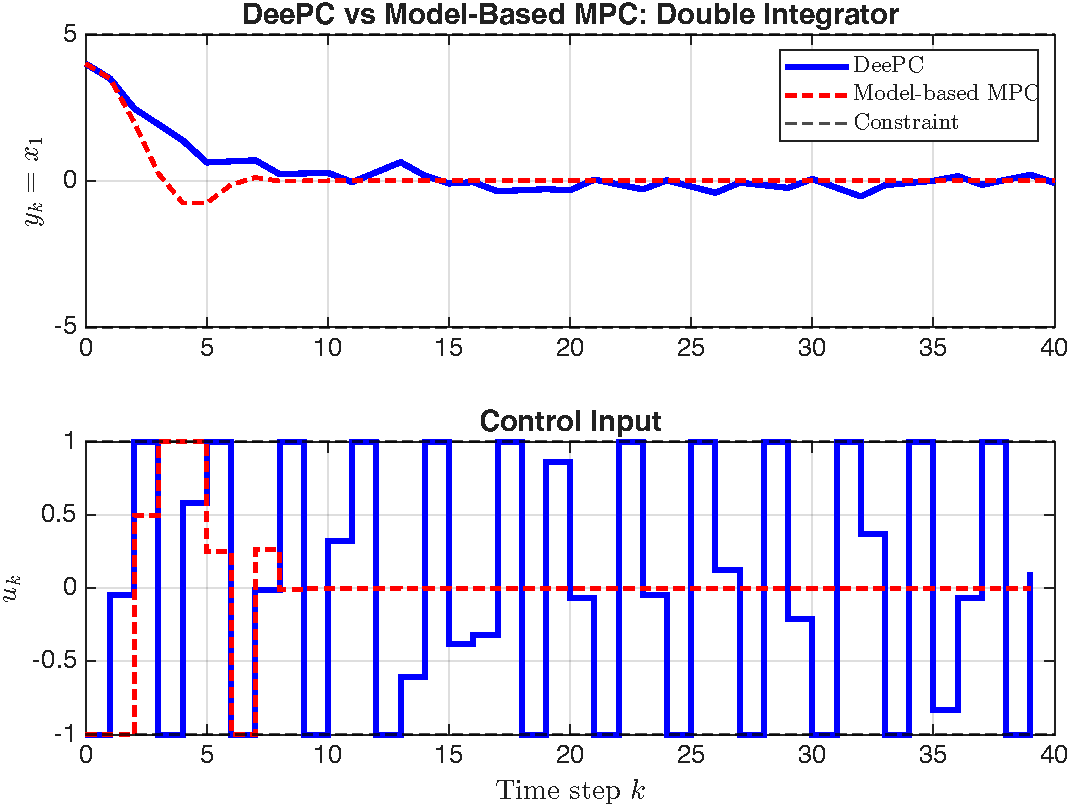
\includegraphics[width=0.88\textwidth]{Figures/fig_deepc_simulation.pdf}
	\caption{DeePC vs model-based MPC for the constrained double integrator. Top: output $y_k = x_1$ regulated from $y_0 = 4$ to the origin. Bottom: control input. The DeePC controller (blue solid) uses 200 data points and Hankel-matrix predictions; the model-based controller (red dashed) uses the known state-space model. Both respect the constraints $|u_k| \le 1$, $|y_k| \le 5$. The DeePC controller shows slightly more aggressive control switching due to finite-data effects and regularisation, while the model-based controller produces a smoother response.}
	\label{fig:deepc_simulation}
\end{figure}

Figure~\ref{fig:deepc_architecture} illustrates the DeePC control loop. The key distinction from model-based MPC is that no system matrices appear anywhere---the Hankel matrices built from raw data serve as the prediction engine.

\begin{figure}[ht]
	\centering
	\begin{tikzpicture}[
		>=Stealth,
		node distance=1.0cm and 1.5cm,
		block/.style={draw, rounded corners=3pt, fill=blue!8,
			minimum width=3.0cm, minimum height=1.0cm, align=center, font=\small},
		blockdata/.style={draw, rounded corners=3pt, fill=orange!15,
			minimum width=3.2cm, minimum height=1.0cm, align=center, font=\small},
		blockplant/.style={draw, rounded corners=3pt, fill=green!10,
			minimum width=2.6cm, minimum height=1.0cm, align=center, font=\small},
		buf/.style={draw, rounded corners=2pt, fill=yellow!15,
			minimum width=2.4cm, minimum height=0.8cm, align=center, font=\small},
		arr/.style={->, thick},
	]
		% Data collection (offline)
		\node[blockdata] (hankel) {Hankel Matrices\\$U_p, Y_p, U_f, Y_f$};
		\node[above=0.4cm of hankel, font=\scriptsize\itshape, text=gray] {Offline: from PE data};

		% DeePC QP
		\node[block, right=2.0cm of hankel] (qp) {DeePC QP\\{\scriptsize solve for $g^*$}};

		% Plant
		\node[blockplant, right=2.0cm of qp] (plant) {True Plant};

		% Past buffer
		\node[buf, below=2.0cm of qp] (buf) {Past Buffer\\$u_\text{ini},\; y_\text{ini}$};

		% Arrows
		\draw[arr] (hankel.east) -- node[above, font=\small] {data} (qp.west);
		\draw[arr] (qp.east) -- node[above, font=\small] {$u_0^*$} (plant.west);
		\draw[arr] (plant.south) -- (plant.south |- buf.east) -- node[above, font=\small] {$y_k$ (measured)} (buf.east);
		\draw[arr] (buf.north) -- node[left, font=\small] {$u_\text{ini}, y_\text{ini}$} (qp.south);

		% Receding horizon annotation
		\draw[arr, dashed, gray] (qp.north) -- ++(0,0.8) -| node[above, pos=0.35, font=\scriptsize\itshape, text=gray] {shift buffer, repeat} (plant.north);
	\end{tikzpicture}
	\caption{DeePC receding-horizon control loop. The Hankel matrices are built once from a persistently exciting offline experiment. At each online step, the past input--output buffer $(u_\text{ini}, y_\text{ini})$ is fed into the DeePC QP along with the Hankel data. The QP finds the optimal combination vector $g^*$, from which the first future input $u_0^*$ is applied to the plant. After measuring the new output, the past buffer is shifted forward and the process repeats.}
	\label{fig:deepc_architecture}
\end{figure}

\subsection{Practical Considerations}
\label{sec:deepc_practical}

For nonlinear systems, the Fundamental Lemma does not hold---the Hankel columns span only LTI behaviours. Workarounds include short rolling data windows (re-collecting data periodically), strong regularisation ($\lambda_g \gg 0$), and multiple shooting with data-driven predictors.

Figure~\ref{fig:deepc_noise} illustrates how measurement noise degrades DeePC performance. As the noise level $\sigma$ increases, the closed-loop trajectory degrades---highlighting the importance of regularisation ($\lambda_g$, $\lambda_\sigma$) when working with noisy data.

\begin{figure}[ht]
	\centering
	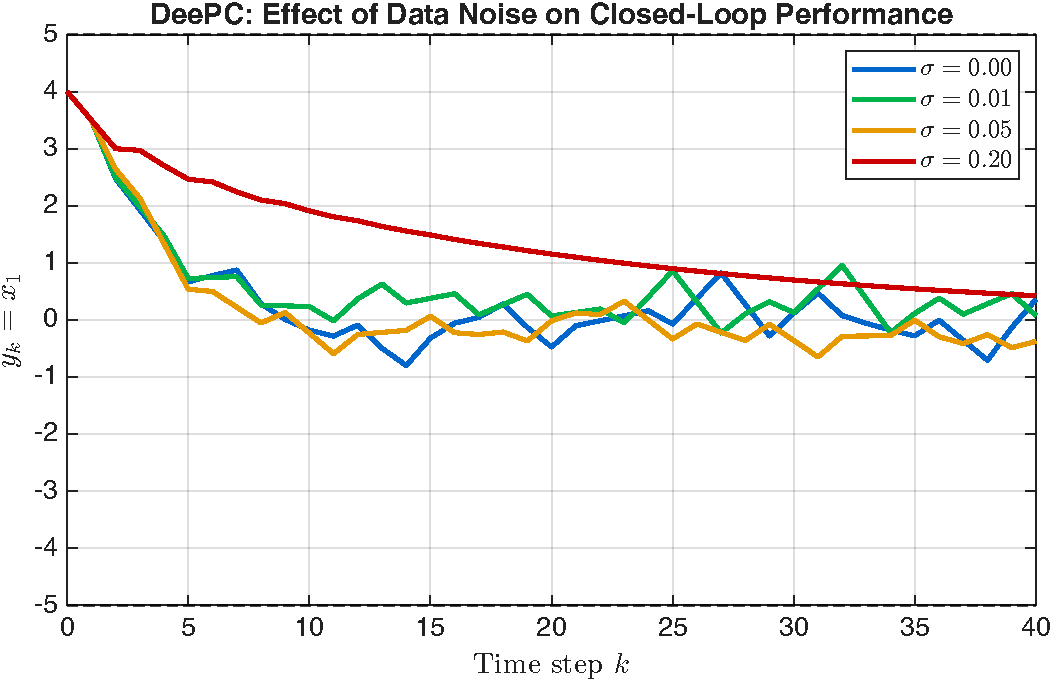
\includegraphics[width=0.85\textwidth]{Figures/fig_deepc_noise.pdf}
	\caption{DeePC noise sensitivity study for the double integrator. Four noise levels are compared: $\sigma = 0$ (noise-free, blue), $\sigma = 0.01$ (green), $\sigma = 0.05$ (orange), and $\sigma = 0.20$ (red). The regularisation weight $\lambda_g$ is scaled with the noise level. At low noise, DeePC closely matches model-based MPC. As noise increases, the Hankel data becomes less representative of the true system, causing slower convergence and larger tracking errors. Data quality and regularisation tuning are essential for reliable DeePC performance.}
	\label{fig:deepc_noise}
\end{figure}


%% ============================================================
%%  SECTION 5: LEARNING MPC (LMPC)
%% ============================================================
\section{Learning MPC}
\label{sec:lmpc}

The methods above learn a model (GP-MPC, Koopman) or bypass it (DeePC) using offline data. Learning MPC (LMPC) takes a different approach: it learns from \emph{repeated executions of the same task}, improving the controller with each iteration.

\subsection{The Iterative Task Setting}
\label{sec:lmpc_setting}

\begin{defnbox}{Definition: Iterative Task}
	A task is \emph{iterative} if the system must repeatedly drive from a fixed initial state $x_S$ to a fixed terminal state $x_F$, under the same dynamics $x_{k+1} = f(x_k, u_k)$ and the same constraints $x_k \in \mathcal{X}$, $u_k \in \mathcal{U}$.
\end{defnbox}

Motivating examples:
\begin{itemize}[noitemsep]
	\item \emph{Autonomous racing.} A car completes laps on the same track. Each lap is an iteration.
	\item \emph{Pick-and-place robots.} A robotic arm repeatedly moves objects between the same two positions.
	\item \emph{Batch chemical processes.} The same reaction is run repeatedly, aiming for a target yield.
\end{itemize}

We index iterations by $j = 0, 1, 2, \ldots$ and time steps within an iteration by $k = 0, 1, \ldots, T_j$, where $T_j$ is the time at which iteration $j$ terminates (i.e.\ $x_{T_j}^{(j)} = x_F$). The trajectory at iteration $j$ is $\{x_0^{(j)}, u_0^{(j)}, x_1^{(j)}, u_1^{(j)}, \ldots, x_{T_j}^{(j)}\}$.


\subsection{Safe Set and Terminal Cost from Data}
\label{sec:lmpc_safe_set}

After $j$ successful iterations, we have $j+1$ complete trajectories (iterations $0, 1, \ldots, j$) that all satisfy the constraints and reach the target. The union of \emph{every state visited during any of these iterations} forms the \emph{sampled safe set}:
\begin{equation}\label{eq:safe_set}
	\mathcal{SS}^j = \bigcup_{i=0}^{j}\bigl\{x_0^{(i)},\; x_1^{(i)},\; \ldots,\; x_{T_i}^{(i)}\bigr\}
\end{equation}
Here $x_k^{(i)}$ denotes the state at time step $k$ during iteration $i$, and $T_i$ is the number of steps iteration $i$ took to reach the target. The superscript $(i)$ always refers to the iteration index and the subscript to the time index within that iteration. Since every iteration reached $x_F$ safely, every state in $\mathcal{SS}^j$ is a state from which the target is \emph{known to be reachable} without violating constraints --- hence the name ``safe set.'' As we complete more iterations, $\mathcal{SS}^j$ can only grow: $\mathcal{SS}^{j} \supseteq \mathcal{SS}^{j-1}$.

For each state in $\mathcal{SS}^j$, we can compute the \emph{cost-to-go}: the total cost that was actually incurred from that state to the target during the iteration in which it was visited. If the same state $x$ was visited during multiple iterations, we take the cheapest one:
\begin{equation}\label{eq:cost_to_go}
	Q^j(x) = \min_{(i,k):\, x_k^{(i)} = x}\; \sum_{t=k}^{T_i} \ell\bigl(x_t^{(i)},\, u_t^{(i)}\bigr)
\end{equation}
The minimum is over all (iteration, time step) pairs $(i,k)$ for which the system was in state $x$ at step $k$ of iteration $i$. The sum counts the stage costs from that point onwards until the end of that iteration. For example, if $\ell = 1$ (minimum-time), then $Q^j(x_k^{(i)}) = T_i - k$: the number of remaining steps. If the same state appeared in a later, faster iteration, $Q^j$ takes the smaller value.

The LMPC optimisation at iteration $j+1$ is:
\begin{equation}\label{eq:lmpc_opt}
	\min_{u_0, \ldots, u_{N-1}}\; \sum_{k=0}^{N-1}\ell(x_k, u_k) + Q^j(x_N)
\end{equation}
subject to:
\begin{align*}
	\text{Initialisation:} \quad & x_0 = x(t) \\
	\text{Dynamics:} \quad & x_{k+1} = f(x_k, u_k) \\
	\text{Constraints:} \quad & x_k \in \mathcal{X}, \quad u_k \in \mathcal{U} \\
	\text{Terminal constraint:} \quad & x_N \in \text{conv}(\mathcal{SS}^j)
\end{align*}
where $\text{conv}(\mathcal{SS}^j)$ denotes the convex hull of the sampled safe set. In practice, the terminal constraint is implemented via convex combination variables: $x_N = \sum_{(i,k)} \lambda_k^{(i)}\,x_k^{(i)}$, with $\lambda_k^{(i)} \ge 0$ and $\sum \lambda = 1$. The terminal cost is interpolated accordingly: $Q^j(x_N) = \sum \lambda_k^{(i)}\,Q^j(x_k^{(i)})$. This convex-hull relaxation is essential---constraining $x_N$ to lie in the \emph{finite} set $\mathcal{SS}^j$ exactly would make the problem combinatorial. For linear systems, the convex hull preserves feasibility; for nonlinear systems, the safe set is used as a lookup table with nearest-neighbour matching as in the worked example below.

\begin{notebox}{Connection to Terminal Sets (Chapter~7)}
	In standard MPC, the terminal set $\mathcal{X}_f$ and terminal cost $V_f(x)$ are computed offline from the model (typically via the DARE and the maximal positive invariant set). In LMPC, both are built from data:
	\begin{itemize}[noitemsep]
		\item $\mathcal{SS}^j$ plays the role of $\mathcal{X}_f$---it is a set of states from which the target is known to be reachable.
		\item $Q^j(x)$ plays the role of $V_f(x)$---it is a valid upper bound on the true cost-to-go.
	\end{itemize}
	As $j$ grows, $\mathcal{SS}^j$ expands and $Q^j$ decreases, so the controller has more freedom and achieves better performance.
\end{notebox}

\subsection{Guarantees}
\label{sec:lmpc_guarantees}

LMPC provides two important properties without requiring an explicit model:

\emph{Recursive feasibility.} If iteration $j$ was feasible (the system reached $x_F$), then iteration $j+1$ is also feasible. The argument has two parts: (i)~\emph{inter-iteration}: the trajectory from iteration $j$ is contained in $\mathcal{SS}^j$, so it is available as a feasible candidate for iteration $j+1$; (ii)~\emph{intra-iteration}: at each time step within iteration $j+1$, the standard shifted-sequence argument applies---the tail of the previous solution provides a feasible candidate, and its terminal state remains in $\mathcal{SS}^j$ because all successor states from previous iterations are already in the safe set.

\emph{Non-increasing cost.} $J^{(j+1)} \le J^{(j)}$. Since the previous trajectory is feasible, the optimal cost at iteration $j+1$ is at most the cost of the previous trajectory. Strict improvement occurs when the expanded safe set opens up shorter or cheaper paths.

The cost sequence $\{J^{(j)}\}$ is non-increasing and bounded below (by zero), so it converges. For convex problems, convergence is to the global optimum; for nonlinear systems, LMPC may converge to a local optimum depending on the initial trajectory and the horizon $N$.


\subsection{Worked Example: LMPC for a Scalar Minimum-Time Problem}
\label{sec:lmpc_example}

\begin{examplebox}{LMPC: Scalar Minimum-Time Problem}
	\emph{System.} $x_{k+1} = x_k + u_k$, with $|u_k| \le 0.5$.

	\emph{Task.} Drive from $x_0 = 2$ to $x_F = 0$ in minimum time (stage cost $\ell = 1$ per step).

	\emph{Iteration 0: conservative controller.} Use $u_k = -0.3$ (well within the constraint) at every step.
	\[
	\begin{array}{c|c c c c c c c c}
		k & 0 & 1 & 2 & 3 & 4 & 5 & 6 & 7 \\
		\hline
		x_k^{(0)} & 2.0 & 1.7 & 1.4 & 1.1 & 0.8 & 0.5 & 0.2 & -0.1
	\end{array}
	\]
	Cost: $J^{(0)} = 7$ steps.

	\solution

	\emph{Build $\mathcal{SS}^0$ and $Q^0$.} The safe set is $\{2.0,\; 1.7,\; 1.4,\; 1.1,\; 0.8,\; 0.5,\; 0.2,\; 0\}$. The cost-to-go from each state is the number of remaining steps: $Q^0(2.0) = 7$, $Q^0(1.7) = 6$, \ldots, $Q^0(0) = 0$.

	\emph{Iteration 1: LMPC.} With $N = 3$, the LMPC plans from $x_0 = 2$ and requires $x_3 \in \mathcal{SS}^0$. Since the constraint allows $u = -0.5$, the optimiser can reach $x_3 = 0.5$ in 3 steps (using $u = -0.5$ each time). The cost-to-go from $x_3 = 0.5$ is $Q^0(0.5) = 2$, so the planned total cost is $3 + 2 = 5$. This is less than $J^{(0)} = 7$.

	After completing iteration 1, the safe set $\mathcal{SS}^1$ is expanded with the new states, and the cost-to-go $Q^1$ is updated with the lower costs observed.

	\emph{Iteration 2 and beyond.} The safe set grows, the cost-to-go improves, and LMPC converges to the optimal solution: $u_k = -0.5$ for 4 steps, reaching $x_F = 0$ in minimum time $T^* = 4$.

\begin{lstlisting}[language=Matlab, caption={LMPC for scalar minimum-time regulation.}]
% 1. System and Constraints
f = @(x, u) x + u;
u_max = 0.5;
x0 = 2;  xF = 0;
N = 3;   % MPC horizon

% 2. Iteration 0: Conservative Controller (u = -0.3)
x_traj = x0;  u_traj = [];
x_cur = x0;
while abs(x_cur) > 0.02
    if abs(x_cur) > 0.3
        u_app = -0.3 * sign(x_cur);    % conservative
    else
        u_app = -x_cur;                 % drive to zero near origin
    end
    u_app = max(-u_max, min(u_max, u_app));
    x_cur = f(x_cur, u_app);
    x_traj(end+1) = x_cur;
    u_traj(end+1) = u_app;
    if length(u_traj) > 50, break; end  % safety limit
end
fprintf('Iteration 0: %d steps\n', length(u_traj));

% 3. Build Safe Set and Cost-to-Go
SS  = x_traj;              % safe set (states visited)
T0  = length(u_traj);
ctg = T0:-1:0;             % cost-to-go from each state

% 4. LMPC Iterations (greedy one-step search)
n_iter = 5;
costs = zeros(1, n_iter+1);
costs(1) = T0;

for j = 1:n_iter
    x_cur = x0;
    x_j = x_cur;  u_j = [];
    while abs(x_cur) > 0.02
        if abs(x_cur) <= 0.3
            best_u = max(-u_max, min(u_max, -x_cur));
        else
            % Greedy: minimise 1 + Q(x_next) over u
            best_u = -0.3*sign(x_cur);  best_cost = 1e6;
            u_grid = linspace(-u_max, u_max, 201);
            for ii = 1:length(u_grid)
                x_next = f(x_cur, u_grid(ii));
                [d, idx] = min(abs(SS - x_next));
                if d < 0.15
                    c_try = 1 + ctg(idx);
                    if c_try < best_cost
                        best_cost = c_try;
                        best_u = u_grid(ii);
                    end
                end
            end
        end
        u_j(end+1) = best_u;
        x_cur = f(x_cur, best_u);
        x_j(end+1) = x_cur;
        if length(u_j) > 30, break; end
    end
    costs(j+1) = length(u_j);
    % Update safe set and cost-to-go (in-place)
    Tj = length(u_j);
    new_ctg = Tj:-1:0;
    for s = 1:length(x_j)
        [d, idx] = min(abs(SS - x_j(s)));
        if d < 0.02
            ctg(idx) = min(ctg(idx), new_ctg(s));
        else
            SS(end+1) = x_j(s);
            ctg(end+1) = new_ctg(s);
        end
    end
    fprintf('Iteration %d: %d steps\n', j, length(u_j));
end

% 5. Plot Cost vs Iteration
figure; bar(0:n_iter, costs, 'FaceColor', [0.2 0.5 0.8]);
xlabel('Iteration j'); ylabel('Steps to reach x_F = 0');
title('LMPC: Cost Improvement Over Iterations'); grid on;
\end{lstlisting}
\end{examplebox}

Figure~\ref{fig:lmpc_iterations} shows the LMPC results over multiple iterations. Iteration~0 (conservative) takes 7~steps. From iteration~1 onward, the controller exploits the expanded safe set and converges to the optimal 4-step trajectory ($u = -0.5$ at every step). The cost (right) decreases monotonically.

\begin{figure}[ht]
	\centering
	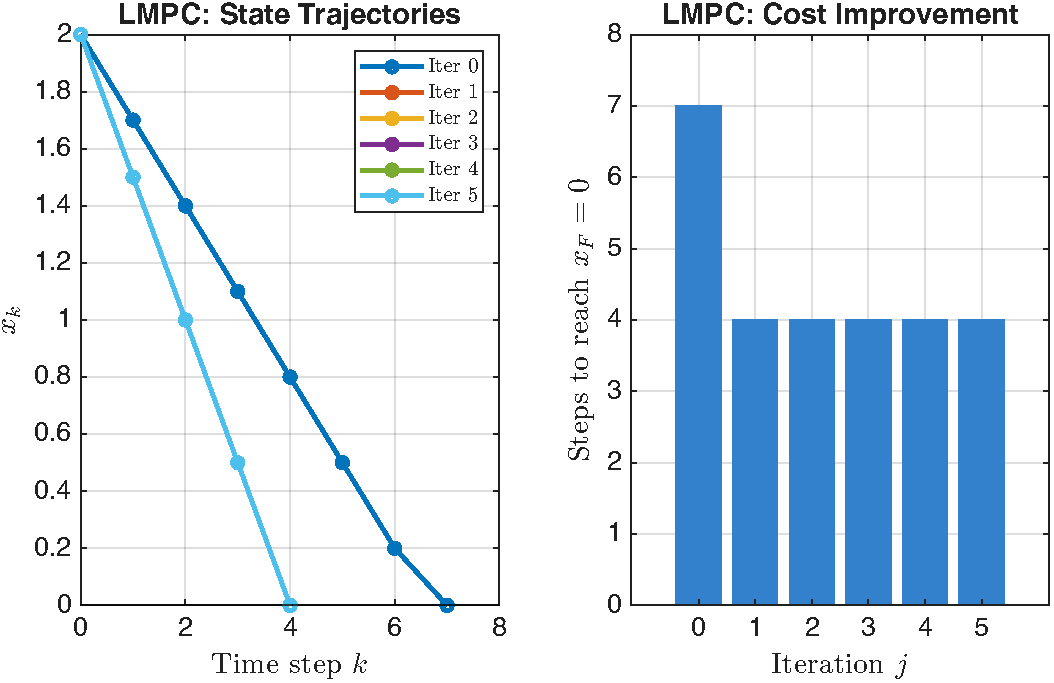
\includegraphics[width=0.92\textwidth]{Figures/fig_lmpc_iterations.pdf}
	\caption{LMPC for the scalar minimum-time problem ($x_{k+1} = x_k + u_k$, $|u_k| \le 0.5$, $x_0 = 2$). Left: state trajectories for iterations~0--5. Iteration~0 (conservative, $u = -0.3$) takes 7~steps. Iterations~1--5 converge to the optimal trajectory using $u = -0.5$ at every step, reaching the origin in~4~steps. Right: the cost (number of steps) decreases monotonically, converging to the theoretical minimum of~4.}
	\label{fig:lmpc_iterations}
\end{figure}


%% ============================================================
%%  WORKED EXAMPLE 2: NN-MPC AUTONOMOUS RACING
%% ============================================================

\subsection{Worked Example: Autonomous Racing with NN-MPC}
\label{sec:nnmpc_racing}

The scalar example above illustrates the LMPC mechanism on a minimal system. We now apply the same principles---safe set expansion, cost-to-go approximation, and iterative improvement---to a realistic nonlinear control problem: \emph{time-optimal autonomous racing} with a dynamic bicycle model and Pacejka tyre forces.

The key departure from the standard LMPC formulation is that the cost-to-go $Q^j$ and the terminal constraint $x_N \in \text{conv}(\mathcal{SS}^j)$ are both approximated by neural networks. This avoids the combinatorial nearest-neighbour search over a growing safe set and provides smooth, differentiable approximations that scale to high-dimensional state spaces.

\subsubsection{Vehicle Model}

The vehicle is modelled as a rear-wheel-drive dynamic bicycle with six states and two inputs:
\begin{equation}\label{eq:racing_state}
	\mathbf{x} = \begin{bmatrix} X \\ Y \\ \varphi \\ v_x \\ v_y \\ r \end{bmatrix}, \qquad
	\mathbf{u} = \begin{bmatrix} \delta \\ D \end{bmatrix},
\end{equation}
where $(X, Y)$ is the position in the global frame, $\varphi$ is the heading angle, $v_x$ and $v_y$ are the longitudinal and lateral velocities in the body frame, $r$ is the yaw rate, $\delta$ is the front steering angle, and $D \in [-1, 1]$ is the normalised throttle/brake command.

The continuous-time dynamics are:
\begin{equation}\label{eq:racing_dynamics}
	\begin{aligned}
		\dot X &= v_x \cos\varphi - v_y \sin\varphi, \\
		\dot Y &= v_x \sin\varphi + v_y \cos\varphi, \\
		\dot\varphi &= r, \\
		\dot v_x &= \tfrac{1}{m}\bigl[F_{rx} - F_{fy}\sin\delta + m\,v_y\,r - F_{\mathrm{drag}}\bigr], \\
		\dot v_y &= \tfrac{1}{m}\bigl[F_{ry} + F_{fy}\cos\delta - m\,v_x\,r\bigr], \\
		\dot r &= \tfrac{1}{I_z}\bigl[F_{fy}\,l_f\cos\delta - F_{ry}\,l_r\bigr].
	\end{aligned}
\end{equation}
Here $m$ is the vehicle mass, $I_z$ the yaw moment of inertia, and $l_f$, $l_r$ the distances from the centre of gravity to the front and rear axles respectively.

\paragraph{Tyre forces.} The lateral tyre forces follow the \emph{Pacejka Magic Formula}~\cite{pacejka2012}. The front and rear slip angles are
\begin{equation}\label{eq:slip_angles}
	\alpha_f = -\arctan\!\frac{v_y + r\,l_f}{v_x} + \delta, \qquad
	\alpha_r = -\arctan\!\frac{v_y - r\,l_r}{v_x},
\end{equation}
and the corresponding lateral forces are
\begin{equation}\label{eq:pacejka}
	F_{fy} = D_f \sin\!\bigl(C_f \arctan(B_f\,\alpha_f)\bigr), \qquad
	F_{ry} = D_r \sin\!\bigl(C_r \arctan(B_r\,\alpha_r)\bigr).
\end{equation}
The longitudinal driving force and drag are modelled as
\begin{equation}\label{eq:drive_drag}
	F_{rx} = C_{m1}\,D - C_{m2}\,D\,v_x, \qquad
	F_{\mathrm{drag}} = C_{r0} + C_{r2}\,v_x^2,
\end{equation}
where $C_{m1}$, $C_{m2}$ capture the motor torque curve and $C_{r0}$, $C_{r2}$ account for rolling resistance and aerodynamic drag. The parameters used in the simulation are listed in Table~\ref{tab:racing_params}.

\begin{table}[ht]
	\centering
	\caption{Vehicle parameters for the racing example.}
	\label{tab:racing_params}
	\begin{tabular}{llrl}
		\toprule
		\textbf{Parameter} & \textbf{Symbol} & \textbf{Value} & \textbf{Unit} \\
		\midrule
		Mass & $m$ & 800 & kg \\
		Yaw inertia & $I_z$ & 1200 & $\text{kg}\cdot\text{m}^2$ \\
		Front axle distance & $l_f$ & 1.2 & m \\
		Rear axle distance & $l_r$ & 1.3 & m \\
		Pacejka front & $B_f,\, C_f,\, D_f$ & $10,\; 1.3,\; 5000$ & $-,\; -,\; \text{N}$ \\
		Pacejka rear & $B_r,\, C_r,\, D_r$ & $11,\; 1.3,\; 7000$ & $-,\; -,\; \text{N}$ \\
		Motor model & $C_{m1},\, C_{m2}$ & $5000,\; 100$ & N, N$\cdot$s/m \\
		Drag model & $C_{r0},\, C_{r2}$ & $50,\; 0.3$ & N, N$\cdot$s$^2$/m$^2$ \\
		Max steering & $\delta_{\max}$ & 0.45 & rad \\
		Throttle range & $D$ & $[-1,\; 1]$ & -- \\
		Speed bounds & $v_x$ & $[0.5,\; 20]$ & m/s \\
		\bottomrule
	\end{tabular}
\end{table}

The dynamics~\eqref{eq:racing_dynamics} are integrated using fourth-order Runge--Kutta with a time step of $\Delta t = 0.05$\,s.


\subsubsection{Track Representation}

The track centreline is constructed as a closed Catmull--Rom spline through 13 waypoints, yielding a circuit of approximately 212\,m. The centreline is parameterised by arc length $s \in [0, L)$, where $L$ is the total track length. At each point, the unit tangent $\mathbf{t}(s)$ and outward normal $\mathbf{n}(s)$ are computed from the spline derivatives, and the local curvature $\kappa(s)$ is obtained from the rate of change of the tangent angle:
\begin{equation}\label{eq:curvature}
	\kappa(s) = \left|\frac{\mathrm{d}\varphi_{\mathrm{tan}}}{\mathrm{d}s}\right|.
\end{equation}
The track boundaries lie at distance $\pm w$ from the centreline along the normal, where $w = 5$\,m is the track half-width.


\subsubsection{Iterative Learning Architecture}
\label{sec:racing_architecture}

The algorithm follows the LMPC paradigm of Section~\ref{sec:lmpc}: iterate between driving and learning, with each lap producing data that improves the next. Two neural networks replace the explicit safe set lookup and convex-hull terminal constraint of the standard LMPC:

\begin{enumerate}
	\item A \textbf{speed map} $v_\theta(s)$ that predicts the target speed at each track position~$s$, replacing the safe-set--based speed targets.
	\item A \textbf{value function} $V_\phi(\mathbf{x})$ that approximates the cost-to-go from any state, replacing the convex-combination terminal cost $Q^j(x_N)$.
\end{enumerate}

\begin{notebox}{Connection to LMPC}
	The speed map encodes the same information as the safe set $\mathcal{SS}^j$: the maximum speed at which the car has been observed to drive safely at each track position. The boost factor $\beta_j$ serves the same purpose as the safe set expansion---it pushes the controller to explore beyond the proven envelope while the curvature cap ensures physical feasibility.
\end{notebox}


\subsubsection{Iteration~0: Data Collection via Pure Pursuit}

The first lap uses a \emph{pure pursuit} controller at a conservative speed $v_{\mathrm{PP}} = 5$\,m/s to complete one full circuit safely. The pure pursuit law computes a lookahead point on the centreline at distance
\begin{equation}\label{eq:lookahead}
	d_{\mathrm{look}} = \max(4\,\text{m},\; 0.9\,v_x)
\end{equation}
ahead of the current arc-length position, then steers towards it. Figure~\ref{fig:nnmpc_pure_pursuit} illustrates the geometry.

\begin{figure}[ht]
	\centering
	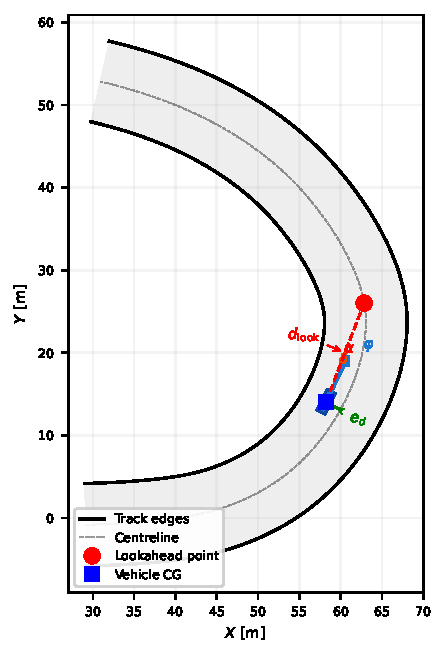
\includegraphics[width=0.65\textwidth]{Figures/fig_nnmpc_pure_pursuit.pdf}
	\caption{Pure pursuit steering geometry. The controller places a lookahead point on the centreline at distance $d_{\mathrm{look}}$ ahead of the vehicle and computes the steering angle $\delta$ from the angle $\alpha$ to that point. If the vehicle drifts off-centre (lateral error $e_d > 0$), the angle $\alpha$ increases and the resulting steering correction pulls the vehicle back towards the centreline.}
	\label{fig:nnmpc_pure_pursuit}
\end{figure}

Let $\alpha$ denote the angle between the vehicle heading and the direction to the lookahead point, and let $d$ be the Euclidean distance to it. The required curvature to intercept the lookahead point is $\gamma = 2\sin\alpha / d$, and the steering angle follows from the bicycle kinematic relation:
\begin{equation}\label{eq:pp_steering}
	\delta = \arctan(\gamma \cdot L_{\mathrm{wb}}), \qquad |\delta| \le \delta_{\max},
\end{equation}
where $L_{\mathrm{wb}} = l_f + l_r$ is the wheelbase. The throttle command is a proportional controller:
\begin{equation}\label{eq:pp_throttle}
	D = \text{clip}\bigl(0.8\,(v_{\mathrm{target}} - v_x),\; -1,\; 1\bigr).
\end{equation}

This controller is inherently self-correcting: if the vehicle drifts off-centre, the angle $\alpha$ to the lookahead point increases, producing a larger steering correction. At the end of iteration~0, the full trajectory $\{(\mathbf{x}_k^{(0)}, \mathbf{u}_k^{(0)}, s_k^{(0)})\}_{k=0}^{T_0}$ is stored.


\subsubsection{NN Speed Map: Learning How Fast to Drive}
\label{sec:racing_speed_map}

After each completed lap, a neural network learns the optimal speed at each track position. The training data is constructed in four stages, illustrated in Figure~\ref{fig:nnmpc_speed_pipeline}.

\begin{figure}[ht]
	\centering
	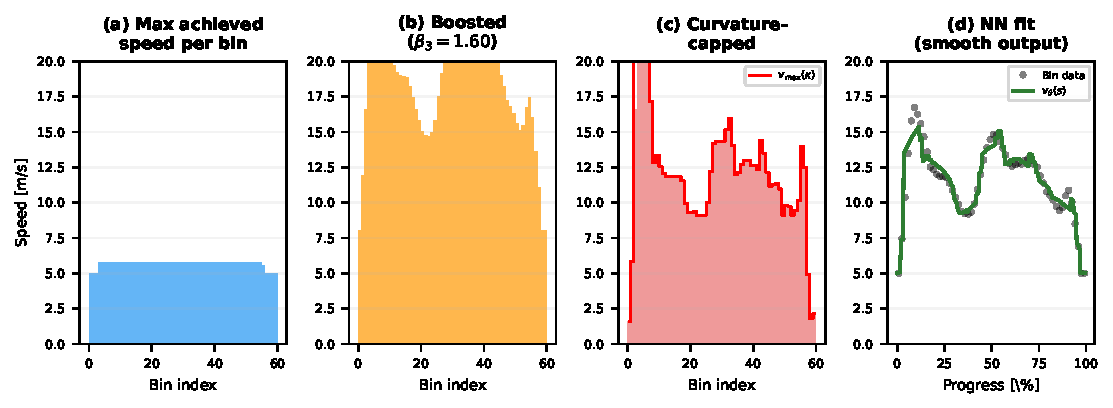
\includegraphics[width=0.95\textwidth]{Figures/fig_nnmpc_speed_pipeline.pdf}
	\caption{NN speed map training pipeline. (a)~The track is divided into $N_{\mathrm{bin}} = 60$ bins and the maximum achieved speed in each bin forms the safe set. (b)~A boost factor $\beta_j$ pushes targets beyond proven speeds. (c)~Curvature-based speed limits cap bins at tight corners. (d)~An \texttt{MLPRegressor} fits a smooth speed profile to the binned data.}
	\label{fig:nnmpc_speed_pipeline}
\end{figure}

\paragraph{Stage~1: Safe set of speeds.} The track is divided into $N_{\mathrm{bin}} = 60$ equal-length bins. For each bin $b$, the maximum longitudinal speed achieved at any point in that bin across all completed iterations is recorded:
\begin{equation}\label{eq:bin_speed}
	\bar{v}_b^{(j)} = \max_{i \le j}\;\max_{k:\, s_k^{(i)} \in \text{bin}\,b}\; v_{x,k}^{(i)}.
\end{equation}
This is the speed-map analogue of the safe set $\mathcal{SS}^j$: the car has been observed driving safely at speed $\bar{v}_b^{(j)}$ in bin $b$.

\paragraph{Stage~2: Iteration-based boost.} To push beyond proven speeds (analogous to safe set expansion), the bin speeds are multiplied by a boost factor that grows with the iteration count:
\begin{equation}\label{eq:boost}
	\tilde{v}_b^{(j)} = \bar{v}_b^{(j)} \cdot \beta_j, \qquad
	\beta_j = \min\!\bigl(1 + 0.15\,(j+1),\; 3.0\bigr).
\end{equation}
This is a controlled extrapolation: at iteration~0, $\beta_0 = 1.15$ (15\% above proven speed); by iteration~7, $\beta_7 = 2.20$. The cap at $3.0$ prevents unbounded growth.

\paragraph{Stage~3: Curvature speed limit.} The boosted targets are capped by the maximum speed that the tyres can sustain through each corner. The steady-state cornering condition requires the lateral acceleration to remain below a threshold $a_{\mathrm{lat,max}}$:
\begin{equation}\label{eq:curv_limit}
	v_{\max}(s) = \sqrt{\frac{a_{\mathrm{lat,max}}}{\kappa(s)}},
\end{equation}
where $\kappa(s)$ is the local curvature. With $a_{\mathrm{lat,max}} = 6\,\text{m/s}^2$, a corner with $\kappa = 0.1\,\text{rad/m}$ limits speed to $\sqrt{60} \approx 7.7$\,m/s. The curvature is smoothed over a window of $\pm 3$ bins to account for the vehicle's spatial extent. Figure~\ref{fig:nnmpc_curvature_speed} shows the curvature profile and the resulting speed limits.

\begin{figure}[ht]
	\centering
	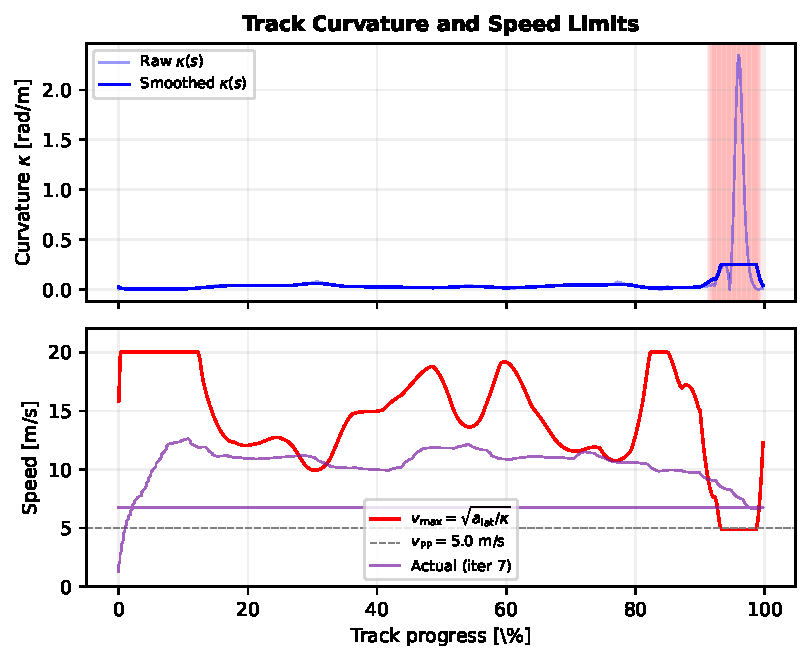
\includegraphics[width=0.7\textwidth]{Figures/fig_nnmpc_curvature_speed.pdf}
	\caption{Top: track curvature $\kappa(s)$ (raw and smoothed). High-curvature zones are shaded. Bottom: curvature-based speed limit $v_{\max} = \sqrt{a_{\mathrm{lat,max}}/\kappa}$ (red), conservative baseline speed $v_{\mathrm{PP}} = 5$\,m/s (dashed grey), and actual speed from the final iteration (purple). The car learns to approach the curvature limit on straights whilst respecting it through corners.}
	\label{fig:nnmpc_curvature_speed}
\end{figure}

The final target speed for each bin combines all three stages:
\begin{equation}\label{eq:target_speed}
	v_{\mathrm{target},b}^{(j)} = \text{clip}\!\left(\min\!\bigl(\tilde{v}_b^{(j)},\; v_{\max,b}\bigr),\; v_{\mathrm{PP}},\; v_{x,\max}\right),
\end{equation}
followed by a 5-bin moving-average smooth to remove discontinuities.

\paragraph{Stage~4: Neural network fit.} An \texttt{MLPRegressor} with two hidden layers of 64 and 32 neurons (\texttt{ReLU} activation) is trained on the binned data. The input features are
\begin{equation}\label{eq:speed_features}
	\mathbf{z}(s) = \left[\frac{s}{L},\;\; \kappa(s),\;\; \sin\!\frac{2\pi s}{L},\;\; \cos\!\frac{2\pi s}{L}\right],
\end{equation}
and the output is the target speed. The Fourier features $\sin(2\pi s/L)$ and $\cos(2\pi s/L)$ encode the periodic (closed-loop) nature of the track, allowing the network to generalise across the start/finish line. The curvature input $\kappa$ provides a direct geometric signal. Five training samples per bin (at uniformly spaced offsets within each bin) give 300 training points in total.


\subsubsection{NN Value Function: Learning the Cost-to-Go}

A second neural network $V_\phi(\mathbf{x})$ approximates the cost-to-go from any state, replacing the convex-combination terminal cost of the standard LMPC~\eqref{eq:lmpc_opt}. With stage cost $\ell = 1$ (minimum-time objective), the cost-to-go from state $\mathbf{x}_k^{(i)}$ is
\begin{equation}\label{eq:vf_target}
	Q^j(\mathbf{x}_k^{(i)}) = T_i - k,
\end{equation}
where $T_i$ is the total number of steps in iteration $i$. Training data from all completed laps is accumulated and the network is retrained after each iteration. The input features are:
\begin{equation}\label{eq:vf_features}
	\mathbf{z}_V(\mathbf{x}) = \left[\frac{X}{50},\;\; \frac{Y}{50},\;\; \cos\varphi,\;\; \sin\varphi,\;\; \frac{v_x}{v_{x,\max}}\right].
\end{equation}
The position is normalised by 50\,m to match the track scale. The heading is encoded as $(\cos\varphi, \sin\varphi)$ to avoid the discontinuity at $\varphi = \pm\pi$. The network architecture is the same as the speed map (two hidden layers of 64 and 32 neurons).


\subsubsection{MPC Controller}
\label{sec:racing_mpc}

At each control step (every $2 \times \Delta t = 0.1$\,s), the controller computes a target speed through four sub-steps:

\paragraph{Step~1: Query the speed map.} The current arc-length position $s$ is obtained by projecting the vehicle position $(X, Y)$ onto the centreline using a KD-tree nearest-neighbour search. The NN speed map returns the target speed:
\begin{equation}\label{eq:mpc_step1}
	v_{\mathrm{target}} = v_\theta(s).
\end{equation}

\paragraph{Step~2: Lookahead braking.} The controller checks the speed map at positions $\Delta t_{\mathrm{look}} \in \{0.5, 1.0, 1.5\}$\,s ahead of the current position. If the target speed is lower ahead (a corner is approaching), the current target is reduced to allow time for deceleration:
\begin{equation}\label{eq:mpc_step2}
	v_{\mathrm{target}} \leftarrow \min\!\Bigl(v_{\mathrm{target}},\;\;
	v_\theta\bigl(s + v_x \cdot \Delta t_{\mathrm{look}}\bigr) + 1.5 \cdot \Delta t_{\mathrm{look}}\Bigr).
\end{equation}
The term $+1.5 \cdot \Delta t_{\mathrm{look}}$ is a deceleration budget: the car may maintain a higher speed now if the corner is still far away. Figure~\ref{fig:nnmpc_lookahead} illustrates this mechanism.

\begin{figure}[ht]
	\centering
	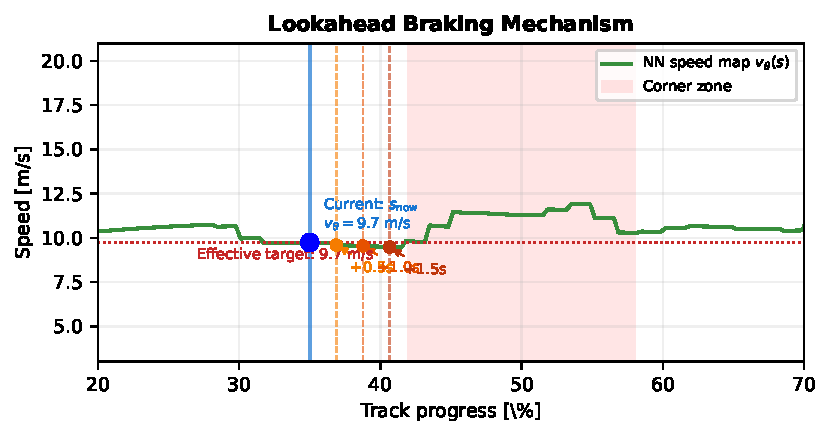
\includegraphics[width=0.7\textwidth]{Figures/fig_nnmpc_lookahead_braking.pdf}
	\caption{Lookahead braking. The controller queries the NN speed map at positions 0.5, 1.0, and 1.5\,s ahead. The corner zone (shaded) has a lower target speed. The effective target at the current position is reduced below the local value $v_\theta(s_{\mathrm{now}})$ to allow proactive deceleration before the corner.}
	\label{fig:nnmpc_lookahead}
\end{figure}

\paragraph{Step~3: Value function adjustment.} The controller evaluates the value function at two hypothetical states: $\mathbf{x}_{\mathrm{fast}}$ with $v_x = v_{\mathrm{target}}$ and $\mathbf{x}_{\mathrm{slow}}$ with $v_x = 0.8\,v_{\mathrm{target}}$. If $V_\phi(\mathbf{x}_{\mathrm{fast}}) < V_\phi(\mathbf{x}_{\mathrm{slow}})$, the faster state leads to lower remaining cost, and the target speed is increased by~5\%:
\begin{equation}\label{eq:mpc_step3}
	v_{\mathrm{target}} \leftarrow
	\begin{cases}
		\min(1.05 \cdot v_{\mathrm{target}},\; v_{x,\max}) & \text{if } V_\phi(\mathbf{x}_{\mathrm{fast}}) < V_\phi(\mathbf{x}_{\mathrm{slow}}), \\
		v_{\mathrm{target}} & \text{otherwise.}
	\end{cases}
\end{equation}

\paragraph{Step~4: Execute.} The computed target speed is passed to the pure pursuit controller~\eqref{eq:pp_steering}--\eqref{eq:pp_throttle}, which returns the steering angle $\delta$ and throttle command~$D$.

Algorithm~\ref{alg:nnmpc} summarises the complete NN-MPC procedure, combining the outer iterative learning loop with the inner control loop.

\begin{algorithm}[ht]
\caption{NN-MPC Iterative Learning for Autonomous Racing}
\label{alg:nnmpc}
\begin{algorithmic}[1]
\Require Track centreline $\{(X(s), Y(s))\}$, vehicle model $f$, number of iterations $J$
\Ensure Trajectories $\{\mathbf{x}^{(j)}, \mathbf{u}^{(j)}\}_{j=0}^{J-1}$ with non-increasing lap times

\Statex \textbf{--- Iteration 0: Data Collection ---}
\State Run one lap with pure pursuit at $v_{\mathrm{PP}} = 5$\,m/s using~\eqref{eq:pp_steering}--\eqref{eq:pp_throttle}
\State Store trajectory $\{(\mathbf{x}_k^{(0)}, \mathbf{u}_k^{(0)}, s_k^{(0)})\}_{k=0}^{T_0}$
\State Initialise safe set $\mathcal{SS}^0$ and cost-to-go $Q^0$

\Statex \textbf{--- Iterations $j = 1, \ldots, J-1$: NN-MPC ---}
\For{$j = 1$ \textbf{to} $J-1$}
    \Statex \quad \textit{Train neural networks:}
    \State Build binned speed targets $\bar{v}_b^{(j)}$ from $\mathcal{SS}^{j-1}$  \hfill \Comment{Eq.~\eqref{eq:bin_speed}}
    \State Apply boost $\hat{v}_b^{(j)} = \bar{v}_b^{(j)} \cdot \beta_j$, cap by curvature $v_{\max}(s)$ \hfill \Comment{Eqs.~\eqref{eq:boost},~\eqref{eq:curv_limit}}
    \State Train speed map $v_\theta(s)$ on binned data \hfill \Comment{MLPRegressor}
    \State Train value function $V_\phi(\mathbf{x})$ on cost-to-go data \hfill \Comment{MLPRegressor}

    \Statex \quad \textit{Run lap with learned controller:}
    \For{each control step ($k = 0, 1, 2, \ldots$) until lap complete}
        \State $v_{\mathrm{target}} \gets v_\theta(s_k)$ \hfill \Comment{Step 1: query speed map}
        \State $v_{\mathrm{target}} \gets \min\!\bigl(v_{\mathrm{target}},\; v_\theta(s_k + v_x \Delta t_{\mathrm{look}}) + 1.5\,\Delta t_{\mathrm{look}}\bigr)$ \hfill \Comment{Step 2: lookahead braking}
        \If{$V_\phi(\mathbf{x}_{\mathrm{fast}}) < V_\phi(\mathbf{x}_{\mathrm{slow}})$} \hfill \Comment{Step 3: value function check}
            \State $v_{\mathrm{target}} \gets \min(1.05 \cdot v_{\mathrm{target}},\; v_{x,\max})$
        \EndIf
        \State Compute $\delta, D$ via pure pursuit~\eqref{eq:pp_steering}--\eqref{eq:pp_throttle} at $v_{\mathrm{target}}$ \hfill \Comment{Step 4: execute}
        \State Apply $(\delta, D)$ to vehicle; integrate dynamics~\eqref{eq:racing_dynamics}
    \EndFor
    \State Store trajectory; update $\mathcal{SS}^j$ and $Q^j$
\EndFor
\end{algorithmic}
\end{algorithm}


\subsubsection{Track-Keeping Mechanisms}

The controller uses no explicit wall or track-boundary constraints. Instead, four complementary mechanisms keep the vehicle within the track:
\begin{enumerate}
	\item \emph{Pure pursuit geometry.} The steering law~\eqref{eq:pp_steering} always aims at a point on the centreline. If the vehicle drifts off-centre, the angle $\alpha$ to the lookahead point increases, producing a larger corrective steering input. This makes the controller inherently self-stabilising.

	\item \emph{Curvature speed limits.} The bound~\eqref{eq:curv_limit} prevents the speed map from requesting speeds that exceed the lateral grip of the tyres. This is the primary mechanism for corner safety.

	\item \emph{Lookahead braking.} The predictive check~\eqref{eq:mpc_step2} ensures the vehicle begins decelerating before reaching a tight corner, rather than reacting only after entering it.

	\item \emph{Off-track abort.} If the lateral deviation from the centreline exceeds $3w$ (15\,m), the lap is aborted. In practice, mechanisms~1--3 keep the deviation below approximately 1.1\,m, well within the 5\,m half-width.
\end{enumerate}


\subsubsection{Safe Set Expansion Over Iterations}

Figure~\ref{fig:nnmpc_safe_set} shows how the safe set grows over iterations. After iteration~0, only a narrow band of states near the centreline has been explored (at 5\,m/s). By iteration~7, the safe set contains over 4\,000 state measurements spanning a wide range of speeds and positions. The colour encodes longitudinal speed---the progression from blue (slow) to red (fast) shows that later iterations reach higher speeds on the straights whilst maintaining safe speeds through corners.

\begin{figure}[ht]
	\centering
	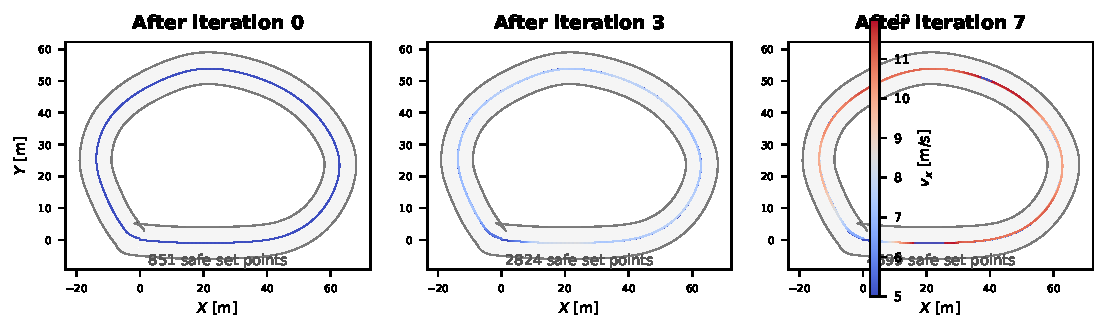
\includegraphics[width=0.95\textwidth]{Figures/fig_nnmpc_safe_set.pdf}
	\caption{Safe set expansion over iterations. Each point is a state visited during a completed lap, coloured by longitudinal speed $v_x$. After iteration~0, only conservative low-speed states are known. By iteration~7, the safe set spans a wide speed range, with higher speeds on straights and lower speeds at corners.}
	\label{fig:nnmpc_safe_set}
\end{figure}


\subsubsection{Simulation Results}

The simulation runs 8~iterations on the custom 13-waypoint track (212\,m). Total computation time is approximately 6\,s on a standard laptop. Figure~\ref{fig:nnmpc_racing_results} presents the results in four panels.

\begin{figure}[ht]
	\centering
	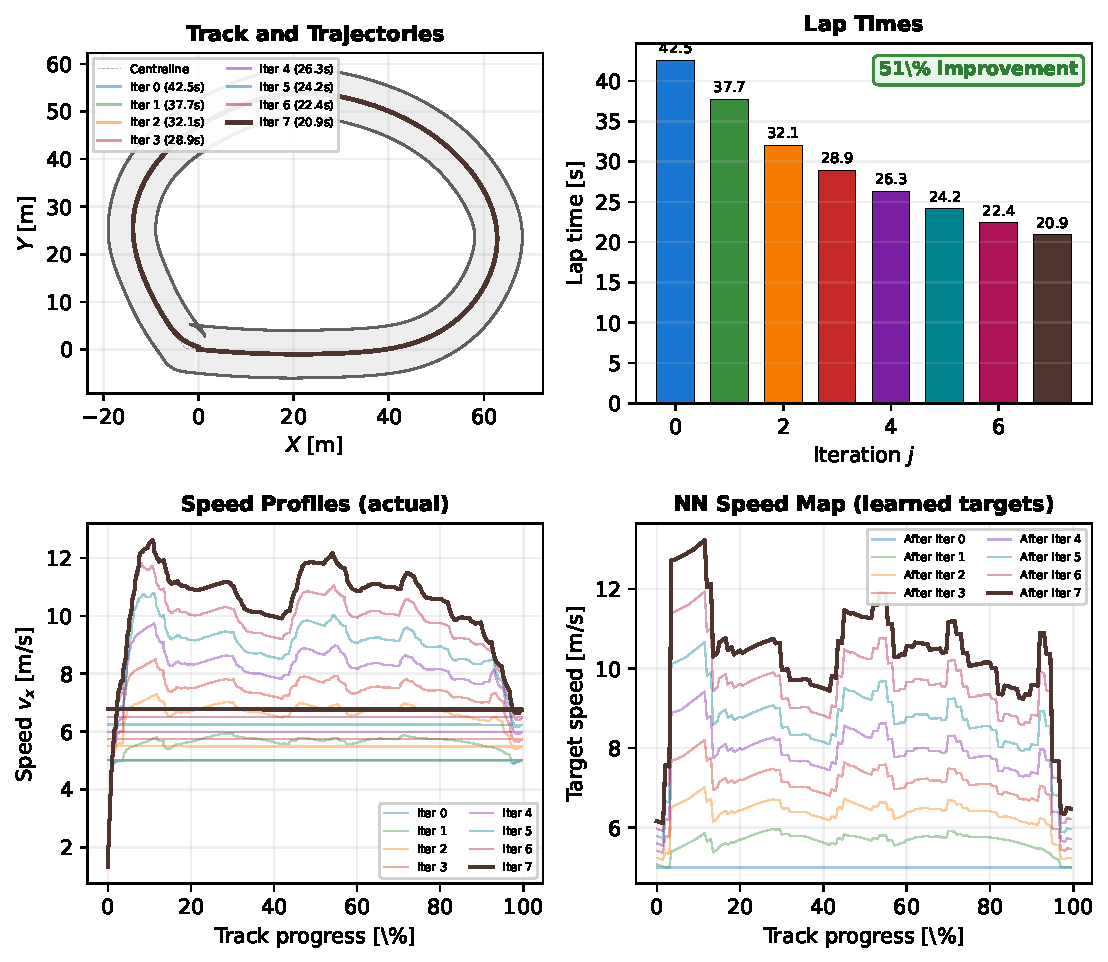
\includegraphics[width=0.95\textwidth]{Figures/fig_nnmpc_racing_results.pdf}
	\caption{NN-MPC autonomous racing results over 8~iterations. Top left: track with overlaid trajectories---later iterations carry higher speed through straights whilst maintaining the racing line through corners. Top right: lap times decrease monotonically from 42.5\,s (pure pursuit at 5\,m/s) to 20.9\,s (NN-MPC at average 10.1\,m/s), a 51\% improvement. Bottom left: actual speed profiles---the car learns to accelerate harder on straights and brake later into corners. Bottom right: NN speed map evolution showing how the learned target speeds increase with each iteration (capped by curvature at corners).}
	\label{fig:nnmpc_racing_results}
\end{figure}

The key observations are:
\begin{itemize}
	\item \emph{Monotone cost decrease.} Lap times decrease from 42.5\,s to 20.9\,s (51\% improvement), consistent with the non-increasing cost property of LMPC (Section~\ref{sec:lmpc_guarantees}).

	\item \emph{Speed profiles.} Iteration~0 drives at a near-constant 5\,m/s. By iteration~7, the car reaches 12.6\,m/s on the straights and brakes to approximately 7\,m/s through tight corners---the curvature speed limit~\eqref{eq:curv_limit} is the binding constraint.

	\item \emph{NN speed map convergence.} The learned speed targets increase rapidly in early iterations and converge as the boost factor saturates and the curvature limits bind. The network produces a smooth, position-dependent speed profile that the pure pursuit controller can track reliably.

	\item \emph{Track safety.} The maximum lateral deviation from the centreline remains below 1.1\,m throughout all 8~iterations. The vehicle never leaves the track.
\end{itemize}

Table~\ref{tab:racing_results} summarises the iteration-by-iteration improvement.

\begin{table}[ht]
	\centering
	\caption{NN-MPC racing results: lap times and average speeds over 8~iterations on the 212\,m track.}
	\label{tab:racing_results}
	\begin{tabular}{crrrc}
		\toprule
		\textbf{Iteration} & \textbf{Lap time [s]} & \textbf{Avg.\ speed [m/s]} & \textbf{Max $|e_d|$ [m]} & \textbf{Controller} \\
		\midrule
		0 & 42.5 & 5.0 & 0.9 & Pure pursuit \\
		1 & 37.7 & 5.6 & 0.9 & NN-MPC \\
		2 & 32.1 & 6.6 & 1.0 & NN-MPC \\
		3 & 28.9 & 7.3 & 1.1 & NN-MPC \\
		4 & 26.3 & 8.0 & 1.1 & NN-MPC \\
		5 & 24.2 & 8.7 & 1.1 & NN-MPC \\
		6 & 22.4 & 9.4 & 1.1 & NN-MPC \\
		7 & 20.9 & 10.1 & 1.1 & NN-MPC \\
		\bottomrule
	\end{tabular}
\end{table}

\begin{alertbox}{Why not solve a full nonlinear MPC online?}
	A ``proper'' LMPC for this system would solve a nonlinear programme with dynamic bicycle constraints at each time step, using the safe set as the terminal constraint. This is computationally demanding---the Pacejka tyre model is highly nonlinear, the state space is six-dimensional, and the safe set grows with every iteration. The NN-MPC approach demonstrated here is a practical approximation: the two neural networks distil the safe set and cost-to-go information into smooth, cheap-to-evaluate functions, and the pure pursuit + proportional speed controller provides a computationally trivial inner loop. The trade-off is that the controller does not optimise a multi-step prediction horizon at each time step---it relies on the NN speed map to encode the optimal speed schedule implicitly. For teaching purposes, this makes the LMPC concept accessible without requiring a browser-based or desktop nonlinear solver.
\end{alertbox}

\begin{notebox}{Running the simulation}
	The companion Python script \texttt{lmpc\_racing.py} implements this example. It requires \texttt{numpy}, \texttt{scipy}, \texttt{scikit-learn}, and \texttt{matplotlib}. Students can modify the \texttt{USER SETTINGS} section to experiment with: the boost factor $\beta_j$ (\texttt{SPEED\_BOOST}), the curvature limit $a_{\mathrm{lat,max}}$ (\texttt{A\_LAT\_MAX}), the network architecture (\texttt{NN\_SPEED\_LAYERS}), the number of iterations, and the track choice (three tracks are included: a 13-waypoint custom circuit and two tracks from the MPCC benchmark~\cite{liniger2015optimization}).

	\medskip
	\textbf{Code:} \url{https://kucukdemiral.github.io/lmpc_racing.py}\\
	\textbf{Colab notebook:} \url{https://kucukdemiral.github.io/lmpc_racing.ipynb}
\end{notebox}


%% ============================================================
%%  SECTION 6: NEURAL NETWORK MODELS IN MPC
%% ============================================================
\section{Neural Network Models in MPC}
\label{sec:nnmpc}

A feedforward neural network can approximate any continuous function to arbitrary accuracy, given enough neurons. This makes it a natural candidate for learning unknown dynamics $x_{k+1} = f_\theta(x_k, u_k)$, where $\theta$ denotes the network weights.

Training is standard: given trajectory data $\{(x_k, u_k, x_{k+1})\}$, minimise the prediction error:
\[
\min_\theta \sum_{k} \|x_{k+1} - f_\theta(x_k, u_k)\|^2
\]
using gradient descent (backpropagation). After training, $f_\theta$ is embedded in the MPC as the prediction model.

\begin{alertbox}{Convexity Structure of Learning-Based MPC}
	A key practical distinction among the methods in this chapter is whether the resulting online optimisation is a convex QP or a non-convex NLP:
	\begin{itemize}[noitemsep]
		\item \emph{Koopman MPC} is a \emph{linear MPC} in the lifted coordinates. The dynamics $z_{k+1} = A_K z_k + B_K u_k$ are linear, the cost is quadratic, and the constraints are linear in the lifted state. The nonlinear lifting $\Psi(x)$ is evaluated only \emph{once} at the measured state to form the initial condition $z_0 = \Psi(x(t))$---a fixed parameter, not a decision variable. The result is a standard QP.
		\item \emph{DeePC} is also a \emph{linear MPC}: the Hankel-matrix constraint is linear in the decision variable $g$, the cost is quadratic, and the $\|\sigma_y\|_2^2$ slack penalty is quadratic. The $\ell_1$ regularisation $\|g\|_1$ is handled by introducing auxiliary variables and linear constraints, so YALMIP reformulates the entire problem as a QP solvable by \texttt{quadprog}.
		\item \emph{GP-MPC} is an NLP. The GP mean $\mu_g(x_k, u_k)$ and variance $\sigma_g^2(x_k, u_k)$ are nonlinear functions of the predicted states, which are decision variables. A common approximation is to evaluate the GP at the \emph{current nominal trajectory} (not the optimised one) and solve a single QP---this is a successive linearisation, not an exact solution.
		\item \emph{NN-MPC} is also an NLP, and typically the most difficult one: neural network activation functions (ReLU, tanh) create a non-smooth, multi-modal landscape with many local minima. A general NLP solver (e.g.\ IPOPT via CasADi) is required.
	\end{itemize}
	In short: Koopman MPC and DeePC preserve the QP structure of standard linear MPC. GP-MPC and NN-MPC do not.
\end{alertbox}

Practical workarounds include:
\begin{itemize}
	\item \emph{Linearise the NN} at each time step (similar to the Real-Time Iteration scheme in Chapter~10), producing a time-varying QP.
	\item \emph{Use the NN for warm-starting}: compute an initial guess with the NN, then refine with a simpler model-based MPC.
	\item \emph{Approximate the MPC policy}: train a NN to clone the MPC controller's input--output map $\pi_\theta(x) \approx u_0^*(x)$, eliminating the online optimisation entirely.
\end{itemize}

The following code demonstrates learning a scalar dynamics model with a simple NN and comparing its predictions to the GP from Section~\ref{sec:gpmpc_example}.

\begin{lstlisting}[language=Matlab, caption={NN dynamics learning for the scalar drag system.}]
% 1. Training Data (same system as GP-MPC example)
rng(0);
T_data = 50;
x_nn = zeros(T_data+1, 1);
u_nn = 2*rand(T_data, 1) - 1;
for k = 1:T_data
    x_nn(k+1) = x_nn(k) + u_nn(k) - 0.2*x_nn(k)^3;
end
X_in  = [x_nn(1:T_data), u_nn];   % inputs: [x_k, u_k]
Y_out = x_nn(2:T_data+1);          % targets: x_{k+1}

% 2. Train a Simple NN (1 hidden layer, 20 neurons)
net = fitnet(20, 'trainlm');
net.trainParam.showWindow = false;
net = train(net, X_in', Y_out');

% 3. Compare Predictions (u = 0)
x_test = linspace(-3, 3, 100);
y_true = x_test + 0 - 0.2*x_test.^3;
y_nn   = net([x_test; zeros(1,100)]);

figure; plot(x_test, y_true, 'r-', 'LineWidth', 2); hold on;
plot(x_test, y_nn, 'b--', 'LineWidth', 2);
xlabel('x_k'); ylabel('x_{k+1}');
legend('True dynamics', 'NN prediction');
title('Neural Network One-Step Prediction (u = 0)'); grid on;
\end{lstlisting}

Figure~\ref{fig:nn_prediction} shows the NN one-step prediction. The NN (blue dashed) captures the nonlinear dynamics well within the training range, though unlike the GP it provides no confidence measure.

\begin{figure}[ht]
	\centering
	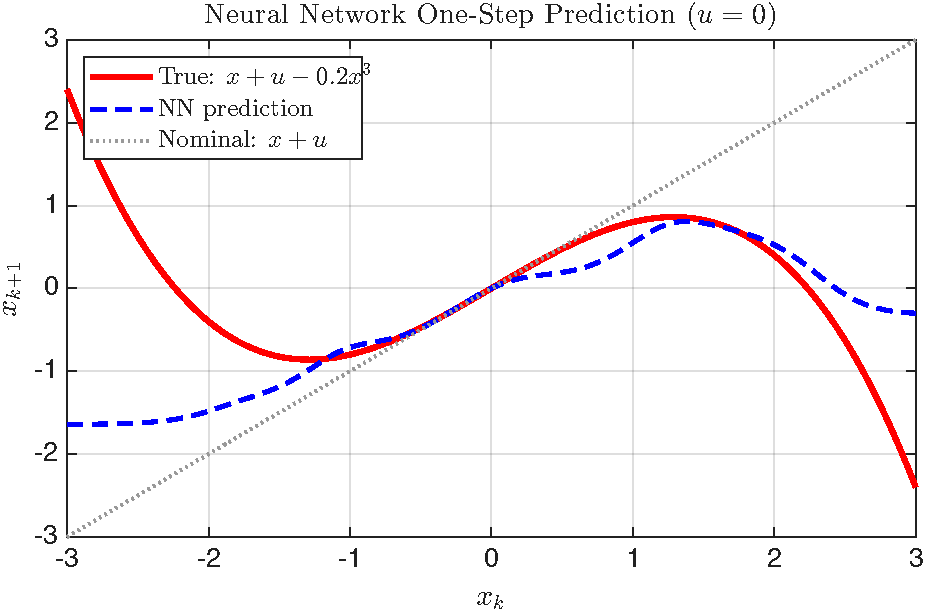
\includegraphics[width=0.82\textwidth]{Figures/fig_nn_prediction.pdf}
	\caption{Neural network one-step prediction for the scalar system $x_{k+1} = x_k + u_k - 0.2\,x_k^3$ (with $u = 0$). A single-hidden-layer NN with 20 neurons (blue dashed) matches the true dynamics (red solid) within the training range $|x| \lesssim 3$. The nominal model $x_{k+1} = x_k$ (grey dotted) ignores the cubic drag entirely. Unlike the GP (Figure~\ref{fig:gp_residual}), the NN provides a point prediction with no uncertainty quantification.}
	\label{fig:nn_prediction}
\end{figure}


%% ============================================================
%%  SECTION 7: REINFORCEMENT LEARNING AND MPC
%% ============================================================
\section{Reinforcement Learning and MPC --- Connections}
\label{sec:rl_mpc}

Reinforcement learning (RL) and MPC solve closely related problems: both seek a policy $\pi(x)$ that minimises cumulative cost (or maximises cumulative reward) over time. The difference is in what is assumed known.

\begin{summarybox}{MPC $\leftrightarrow$ RL Correspondences}
	\begin{center}
		\begin{tabular}{l l}
			\toprule
			\emph{MPC concept} & \emph{RL concept} \\
			\midrule
			Stage cost $\ell(x_k, u_k)$ & Negative reward $-r(s_k, a_k)$ \\
			Terminal cost $V_f(x_N)$ & Value function $V(s)$ \\
			Model $x_{k+1} = f(x_k, u_k)$ & Transition model $P(s'|s, a)$ \\
			Prediction horizon $N$ & Discount factor $\gamma$ (conceptually) \\
			Receding horizon & Model-based replanning \\
			\bottomrule
		\end{tabular}
	\end{center}
\end{summarybox}

Three productive ways to combine RL and MPC:

\emph{1.\ MPC as a structured policy in RL.} Rather than learning a policy from scratch (a neural network mapping states to actions), use the MPC controller $\pi_\text{MPC}(x) = u_0^*(x)$ as the policy. The MPC structure provides constraint satisfaction and stability by construction---RL then tunes the MPC parameters ($Q$, $R$, $N$, or the model itself) to maximise long-term performance.

\emph{2.\ RL for MPC tuning.} The cost matrices $Q$ and $R$ are typically hand-tuned. RL can automate this: treat $Q$ and $R$ as the ``action'' of an outer-loop agent, evaluate the resulting MPC performance over a simulation episode, and update $Q$ and $R$ via policy gradient or Bayesian optimisation.

\emph{3.\ MPC as a safe exploration policy.} During RL training, the agent must explore, which can lead to constraint violations. By using MPC with conservative constraints as the exploration policy, the system remains safe while the RL agent collects data to improve its value function.

\begin{lstlisting}[language=Matlab, caption={RL-style tuning of MPC weight $R$ on a scalar system.}]
% 1. System
A = 1;  B = 1;  Q = 1;  N = 5;  x0 = 3;  T_ep = 20;
f = @(x, u) A*x + B*u;

% 2. Evaluate one episode with given R
run_episode = @(R_val) eval_mpc(A, B, Q, R_val, N, x0, T_ep);

% 3. Grid Search (simple RL: evaluate cost for each R)
R_grid = logspace(-2, 1, 30);
J_grid = zeros(size(R_grid));
for i = 1:length(R_grid)
    J_grid(i) = run_episode(R_grid(i));
end
[J_best, idx] = min(J_grid);
fprintf('Best R = %.3f, Cost = %.2f\n', R_grid(idx), J_best);

figure; semilogx(R_grid, J_grid, 'b-o', 'LineWidth', 2);
xlabel('R (control weight)'); ylabel('Episode cost J');
title('RL-Style Tuning of MPC Weight R'); grid on;

% --- Helper function ---
function J = eval_mpc(A, B, Q, R, N, x0, T_ep)
    P = dare(A, B, Q, R);
    x = x0; J = 0;
    for t = 1:T_ep
        % Simple unconstrained MPC (LQR) for speed
        K = (R + B'*P*B) \ (B'*P*A);
        u = -K * x;
        J = J + Q*x^2 + R*u^2;
        x = A*x + B*u;
    end
    J = J + x'*P*x;
end
\end{lstlisting}


%% ============================================================
%%  SECTION 8: PRACTICAL GUIDELINES
%% ============================================================
\section{Practical Guidelines and Comparison}
\label{sec:comparison}

The choice of method depends on the application context. The decision flowchart in Figure~\ref{fig:method_flowchart} provides a practical guide, and the following questions summarise the logic.

\begin{figure}[ht]
	\centering
	\begin{tikzpicture}[
		>=Stealth,
		node distance=0.9cm and 1.6cm,
		decision/.style={draw, diamond, aspect=2.5, fill=yellow!15,
			minimum width=2.4cm, minimum height=0.9cm, align=center,
			font=\small, inner sep=3pt},
		result/.style={draw, rounded corners=4pt, fill=green!15,
			minimum width=2.4cm, minimum height=0.8cm, align=center,
			font=\small\bfseries},
		arr/.style={->, thick},
		lbl/.style={font=\scriptsize, fill=white, inner sep=2pt},
	]
		% Decision 1: Have a model?
		\node[decision] (d1) {Have a\\model?};

		% Yes branch
		\node[decision, right=4cm of d1] (d2) {Model\\accurate?};
		\draw[arr] (d1.east) -- node[lbl, above] {Yes} (d2.west);

		\node[result, right=2.0cm of d2] (r1) {Standard MPC\\{\scriptsize (Ch.\,7)}};
		\draw[arr] (d2.east) -- node[lbl, above] {Yes} (r1.west);

		\node[decision, below=1.5cm of d2] (d2b) {Uncertainty\\bounded?};
		\draw[arr] (d2.south) -- node[lbl, right] {No} (d2b.north);

		\node[result, right=2.2cm of d2b] (r2) {Tube MPC};
		\draw[arr] (d2b.east) -- node[lbl, above] {Yes} (r2.west);

		\node[result, below=1.2cm of d2b] (r3) {GP-MPC};
		\draw[arr] (d2b.south) -- node[lbl, right] {No} (r3.north);

		% No branch
		\node[decision, below=3.2cm of d1] (d3) {System\\LTI?};
		\draw[arr] (d1.south) -- node[lbl, right] {No} (d3.north);

		\node[result, right=2.2cm of d3] (r4) {DeePC};
		\draw[arr] (d3.east) -- node[lbl, above] {Yes} (r4.west);

		\node[decision, below=1.5cm of d3] (d4) {Mildly\\nonlinear?};
		\draw[arr] (d3.south) -- node[lbl, right] {No} (d4.north);

		\node[result, right=2.2cm of d4] (r5) {Koopman MPC};
		\draw[arr] (d4.east) -- node[lbl, above] {Yes} (r5.west);

		\node[decision, below=1.5cm of d4] (d5) {Repetitive\\task?};
		\draw[arr] (d4.south) -- node[lbl, right] {No} (d5.north);

		\node[result, right=2.2cm of d5] (r6) {LMPC};
		\draw[arr] (d5.east) -- node[lbl, above] {Yes} (r6.west);

		\node[result, below=1.2cm of d5] (r7) {NN-MPC\\{\scriptsize (with caution)}};
		\draw[arr] (d5.south) -- node[lbl, right] {No} (r7.north);
	\end{tikzpicture}
	\caption{Decision flowchart for selecting an MPC method. Starting from the availability of a model, the flowchart guides the practitioner through a sequence of questions about model accuracy, uncertainty structure, system linearity, and task structure. Each terminal node (green) indicates the recommended approach.}
	\label{fig:method_flowchart}
\end{figure}


\begin{summarybox}{Comparison of Learning-Based MPC Methods}
	\begin{center}
		\resizebox{\linewidth}{!}{%
		\small
		\begin{tabular}{l c c c c c}
			\toprule
			& \emph{GP-MPC} & \emph{Koopman} & \emph{DeePC} & \emph{LMPC} & \emph{NN-MPC} \\
			\midrule
			Nominal model needed? & Yes & No & No & Yes & No \\
			System class & Nonlinear & Mildly NL & LTI & Any & Nonlinear \\
			Online computation & NLP (mild) & QP & QP & QP/NLP & NLP (severe) \\
			Uncertainty quantified? & Yes & No & Indirectly & No & No \\
			Guarantees & Chance (1-step) & Approx.\ linear & LTI equiv. & Recur.\ feas. & Weak \\
			YALMIP usable? & Yes & Yes & Yes & Yes & No \\
			\bottomrule
		\end{tabular}%
		}
	\end{center}
\end{summarybox}

\begin{alertbox}{Assumptions and Limitations}
	Every learning-based method introduces assumptions beyond those of standard MPC:
	\begin{itemize}[noitemsep]
		\item GP-MPC assumes the residual is a smooth function (kernel choice).
		\item Koopman MPC assumes the dictionary spans the relevant observables.
		\item DeePC assumes LTI dynamics (or mild nonlinearity with regularisation).
		\item LMPC assumes the task is repetitive with fixed initial and terminal conditions.
		\item NN-MPC provides no formal constraint or stability guarantees.
	\end{itemize}
	The choice of method must be guided by the problem structure, the available data, and the required guarantees.
\end{alertbox}


%% ============================================================
%%  SECTION 9: SUMMARY
%% ============================================================
\section{Summary}
\label{sec:learning_summary}

\begin{summarybox}{Chapter Summary}
	This chapter introduced five methods for combining learning with MPC:
	\begin{enumerate}
		\item \emph{GP-MPC}: learns a probabilistic residual model; provides adaptive constraint tightening via chance constraints.
		\item \emph{Koopman MPC}: lifts nonlinear dynamics to a linear space via a data-driven dictionary; reduces to a standard QP.
		\item \emph{DeePC}: uses raw input--output data in a Hankel-matrix formulation; bypasses system identification entirely.
		\item \emph{LMPC}: exploits data from repeated task executions to expand the safe set and improve performance.
		\item \emph{NN-MPC}: uses neural networks for dynamics learning; expressive but non-convex and harder to certify.
	\end{enumerate}
	The key trade-off is between expressiveness and tractability. Koopman MPC and DeePC preserve the QP structure of standard linear MPC, making them directly suitable for real-time implementation with existing solvers. GP-MPC is an NLP but admits effective convex approximations. NN-MPC is the most expressive but also the least tractable, producing non-convex NLPs with limited formal guarantees.
\end{summarybox}

\subsection*{Further Reading}

\begin{itemize}[noitemsep]
	\item Willems, Rapisarda, Markovsky \& De Moor (2005): the Fundamental Lemma~\cite{Willems2005}.
	\item Rasmussen \& Williams (2006): the standard textbook on Gaussian processes~\cite{Rasmussen2006}.
	\item Hewing, Wabersich, Menner \& Zeilinger (2020): a survey of learning-based MPC~\cite{Hewing2020}.
	\item Coulson, Lygeros \& D\"orfler (2019): the original DeePC paper~\cite{Coulson2019}.
	\item Rosolia \& Borrelli (2018): Learning MPC for iterative tasks~\cite{Rosolia2018}.
	\item Korda \& Mezi\'c (2018): Koopman-based linear predictors for nonlinear MPC~\cite{Korda2018}.
	\item D\"orfler, Coulson \& Markovsky (2023): bridging data-driven and model-based control via regularisation~\cite{Dorfler2023}.
\end{itemize}


%% ============================================================
%%  EXERCISES
%% ============================================================
\section*{Exercises}

\begin{enumerate}
	\item \emph{GP Regression (hand-worked).}
	\begin{enumerate}
		\item Given 4 training points $\{(0, 0.1),\; (1, 0.9),\; (2, 0.15),\; (3, -0.8)\}$ and the SE kernel with $\sigma_f = 1$, $\ell = 1.5$, $\sigma_n = 0.1$, compute the $4 \times 4$ Gram matrix $K$.
		\item Compute the predictive mean $\mu_*$ and variance $\sigma_*^2$ at $x_* = 1.5$.
		\item If this GP models a dynamics residual and the state constraint is $|x| \le 5$, compute the tightened constraint at $x_* = 1.5$ for $\delta = 0.025$ (i.e.\ a 97.5\% chance constraint).
		\item Discuss qualitatively: what happens to $\sigma_*^2$ as the number of training points near $x_*$ increases?
	\end{enumerate}

	\item \emph{EDMD Identification (hand-worked).}
	\begin{enumerate}
		\item For $x_{k+1} = 0.5\,x_k + 0.2\,x_k^2 + u_k$ with dictionary $\Psi(x) = [x,\; x^2]^\top$, generate 6 transitions from $x_0 = 0$ with inputs $u = [0.5,\; -0.3,\; 0.8,\; -0.5,\; 0.1,\; -0.2]$.
		\item Construct the lifted data matrices $Z$, $Z'$, $U$ and solve for $[A_K,\; B_K]$ via the pseudoinverse.
		\item Compare the one-step prediction error of the Koopman model to that of a linearisation about the origin ($x_{k+1} \approx 0.5\,x_k + u_k$) at the test point $x = 2$, $u = 0$.
	\end{enumerate}

	\item \emph{DeePC: Hankel Matrix Construction.}
	\begin{enumerate}
		\item For the first-order system $y_{k+1} = 0.9\,y_k + u_k$ with $T = 10$ data points and $L = 4$, construct the Hankel matrices $\mathcal{H}_4(u^d)$ and $\mathcal{H}_4(y^d)$.
		\item Verify the rank condition for PE of order $L + n = 5$.
		\item Write out the DeePC QP~\eqref{eq:deepc_qp} explicitly (decision variables, cost, constraints) for $T_\text{ini} = 1$, $N = 3$.
		\item Compute the minimum data length $T$ required for PE with system orders $n = 1, 2, 4$ and input dimension $m = 1$, assuming $L = 12$.
	\end{enumerate}

	\item \emph{DeePC vs Model-Based MPC (MATLAB).}
	\begin{enumerate}
		\item Implement DeePC for the double integrator (Section~\ref{sec:deepc_double_int}) using the code provided.
		\item Implement standard model-based MPC (Chapter~7 formulation) for the same system with the same cost matrices and constraints.
		\item Compare the closed-loop trajectories. Are they identical? Explain.
		\item Corrupt the data with additive noise: $u_k^d \leftarrow u_k^d + \varepsilon_k$, $y_k^d \leftarrow y_k^d + \eta_k$, with $\varepsilon_k, \eta_k \sim \mathcal{N}(0, \sigma^2)$ for $\sigma \in \{0.01,\; 0.1,\; 0.5\}$. How does DeePC performance degrade? How do the regularisation parameters $\lambda_g$ and $\lambda_\sigma$ help?
	\end{enumerate}

	\item \emph{LMPC (scalar computation).}
	\begin{enumerate}
		\item For $x_{k+1} = x_k + u_k$, $|u_k| \le 1$, $x_0 = 3$, $x_F = 0$, with stage cost $\ell = 1$: compute the trajectory for iteration~0 using $u_k = -0.5$ at every step.
		\item Construct the safe set $\mathcal{SS}^0$ and the cost-to-go $Q^0(x)$ for each state in the trajectory.
		\item With $N = 2$, show that iteration~1 can achieve $u_k = -1$ (i.e.\ saturated input) and reach the origin faster. Compute the cost $J^{(1)}$.
		\item What is the theoretical minimum cost (minimum number of steps)? How many LMPC iterations are needed to achieve it?
	\end{enumerate}

	\item \emph{Method Selection (conceptual).} For each scenario, argue which learning-based MPC approach is most appropriate and explain your reasoning:
	\begin{enumerate}
		\item A chemical reactor with well-understood reaction kinetics but unknown and time-varying heat loss to the environment.
		\item An autonomous car performing laps on a race circuit, where the track layout is fixed but tyre grip varies with temperature.
		\item A power electronics converter whose input--output behaviour has been measured extensively, and the internal dynamics are believed to be linear.
		\item A soft robotic arm with complex, highly nonlinear dynamics that are difficult to model from first principles.
	\end{enumerate}
\end{enumerate}
